 % chktex-file 13
 % chktex-file 24
 % chktex-file 44
 % chktex-file 1
 \chapter{Experimentelle Erprobung und Evaluierung}\label{ch:anomaliedetektion_test}
Im Folgenden werden die ausgewählten Algorithmen aus~\hyperref[sec:algorithmen]{Abs.~\Ref*{sec:algorithmen}} anhand realer und synthetischer
Daten getestest, evaluiert und gegenübergestellt. Ziel ist es, die Leistungsfähigkeit der verschiedenen Verfahren hinsichtlich ihrer
Erkennungsrate, Robustheit und Effizienz zu untersuchen. Dabei wird zwischen den drei Anomalietypen~–~Punkt-, Subsequenz- und
Korrelationsanomalien~–~unterschieden, um herauszufinden, welche Algorithmen sich besonders für die jeweilige Art von Abweichung eignen.

Zunächst wird die experimentelle Umgebung beschrieben, einschließlich der verwendeten Datensätze und Metriken zur Bewertung der Algorithmen.
Anschließend erfolgt die Durchführung der Experimente, wobei sowohl synthetische als auch reale Sensordaten auf Basis des \ac{sspx1} Systems
verwendet werden. Abschließend wird eine vergleichende Analyse vorgenommen, um Stärken und Schwächen der Algorithmen herauszuarbeiten und
deren Eignung für den praktischen Einsatz in Predictive-Maintenance-Szenarien zu bewerten.

\section{Detektion von Punktanomalien}\label{sec:punktanomaliedetektion}
Zur Erprobung der Punktanomaliedetektionsalgorithmen werden drei, im Original aus den Datenaufzeichnungen der \ac{sspx1} stammende, Ausschnitte 
der Datensätze um einige synthetische Punktanomalien erweitert. Dabei handelt es sich um die \ac{ram} und \ac{cpu} Auslastung sowie die \ac{cpu} Temperatur.
Die Zeitspanne, über die Daten entstanden sind, entspricht einer Dauer von genau 48 Stunden und umfasst ca.~17000 Datenpunkten, wie
in~\hyperref[fig:punktanomalien_testdata]{Abb.~\Ref*{fig:punktanomalien_testdata}} dargestellt ist.

\begin{figure}[t!]
    \centering
        \includegraphics[width=1\linewidth]{ch5_anomalieerkennung/abbildungen/punktanomalien_datensätze.pdf}
    \caption{\centering Drei Datensätze zur Gegenüberstellung und Evaluierung der beiden Algorithmen
    aus~\hyperref[tab:algorithmen]{Tab.~\Ref*{tab:algorithmen}} mit synthetisch eingefügten Anomalien, die plausible Anomaliefälle darstellen.}
~\label{fig:punktanomalien_testdata}
\end{figure}

Für die Parametrisierung der beiden Algorithmen \textbf{\acf{hbos}} und \textbf{\ac{swz}} wurden
jeweils identische Fenstergrößen und Kontaminationsparameter übergeben. Die Kontamination gibt an, welcher relative Anteil eines Datensatzes
anomal ist und ist daher bereits eine Unsicherheit in der Analyse. Jedoch kann dies etwas eingedämmt werden, indem mehrere Durchläufe mit
variabler Kontamination durchgeführt werden. Für die Tests der drei Datensätze wurden jeweils Kontaminationswerte von 0,02 \%, 0,069 \% und
0,1 \% verwendet. Die genaue Kontamination entspricht den 0,069 \%, da 12 aus den insgesamt jeweils 17281 Datenpunkten eine Anomalie
darstellen. Bei der Analyse von Punktanomalien kann generell eine geringere Kontamination angenommen werden, da es sich nur um vereinzelte,
punktuelle Ausreißer handelt.

\begin{figure}[b!]
    \centering
        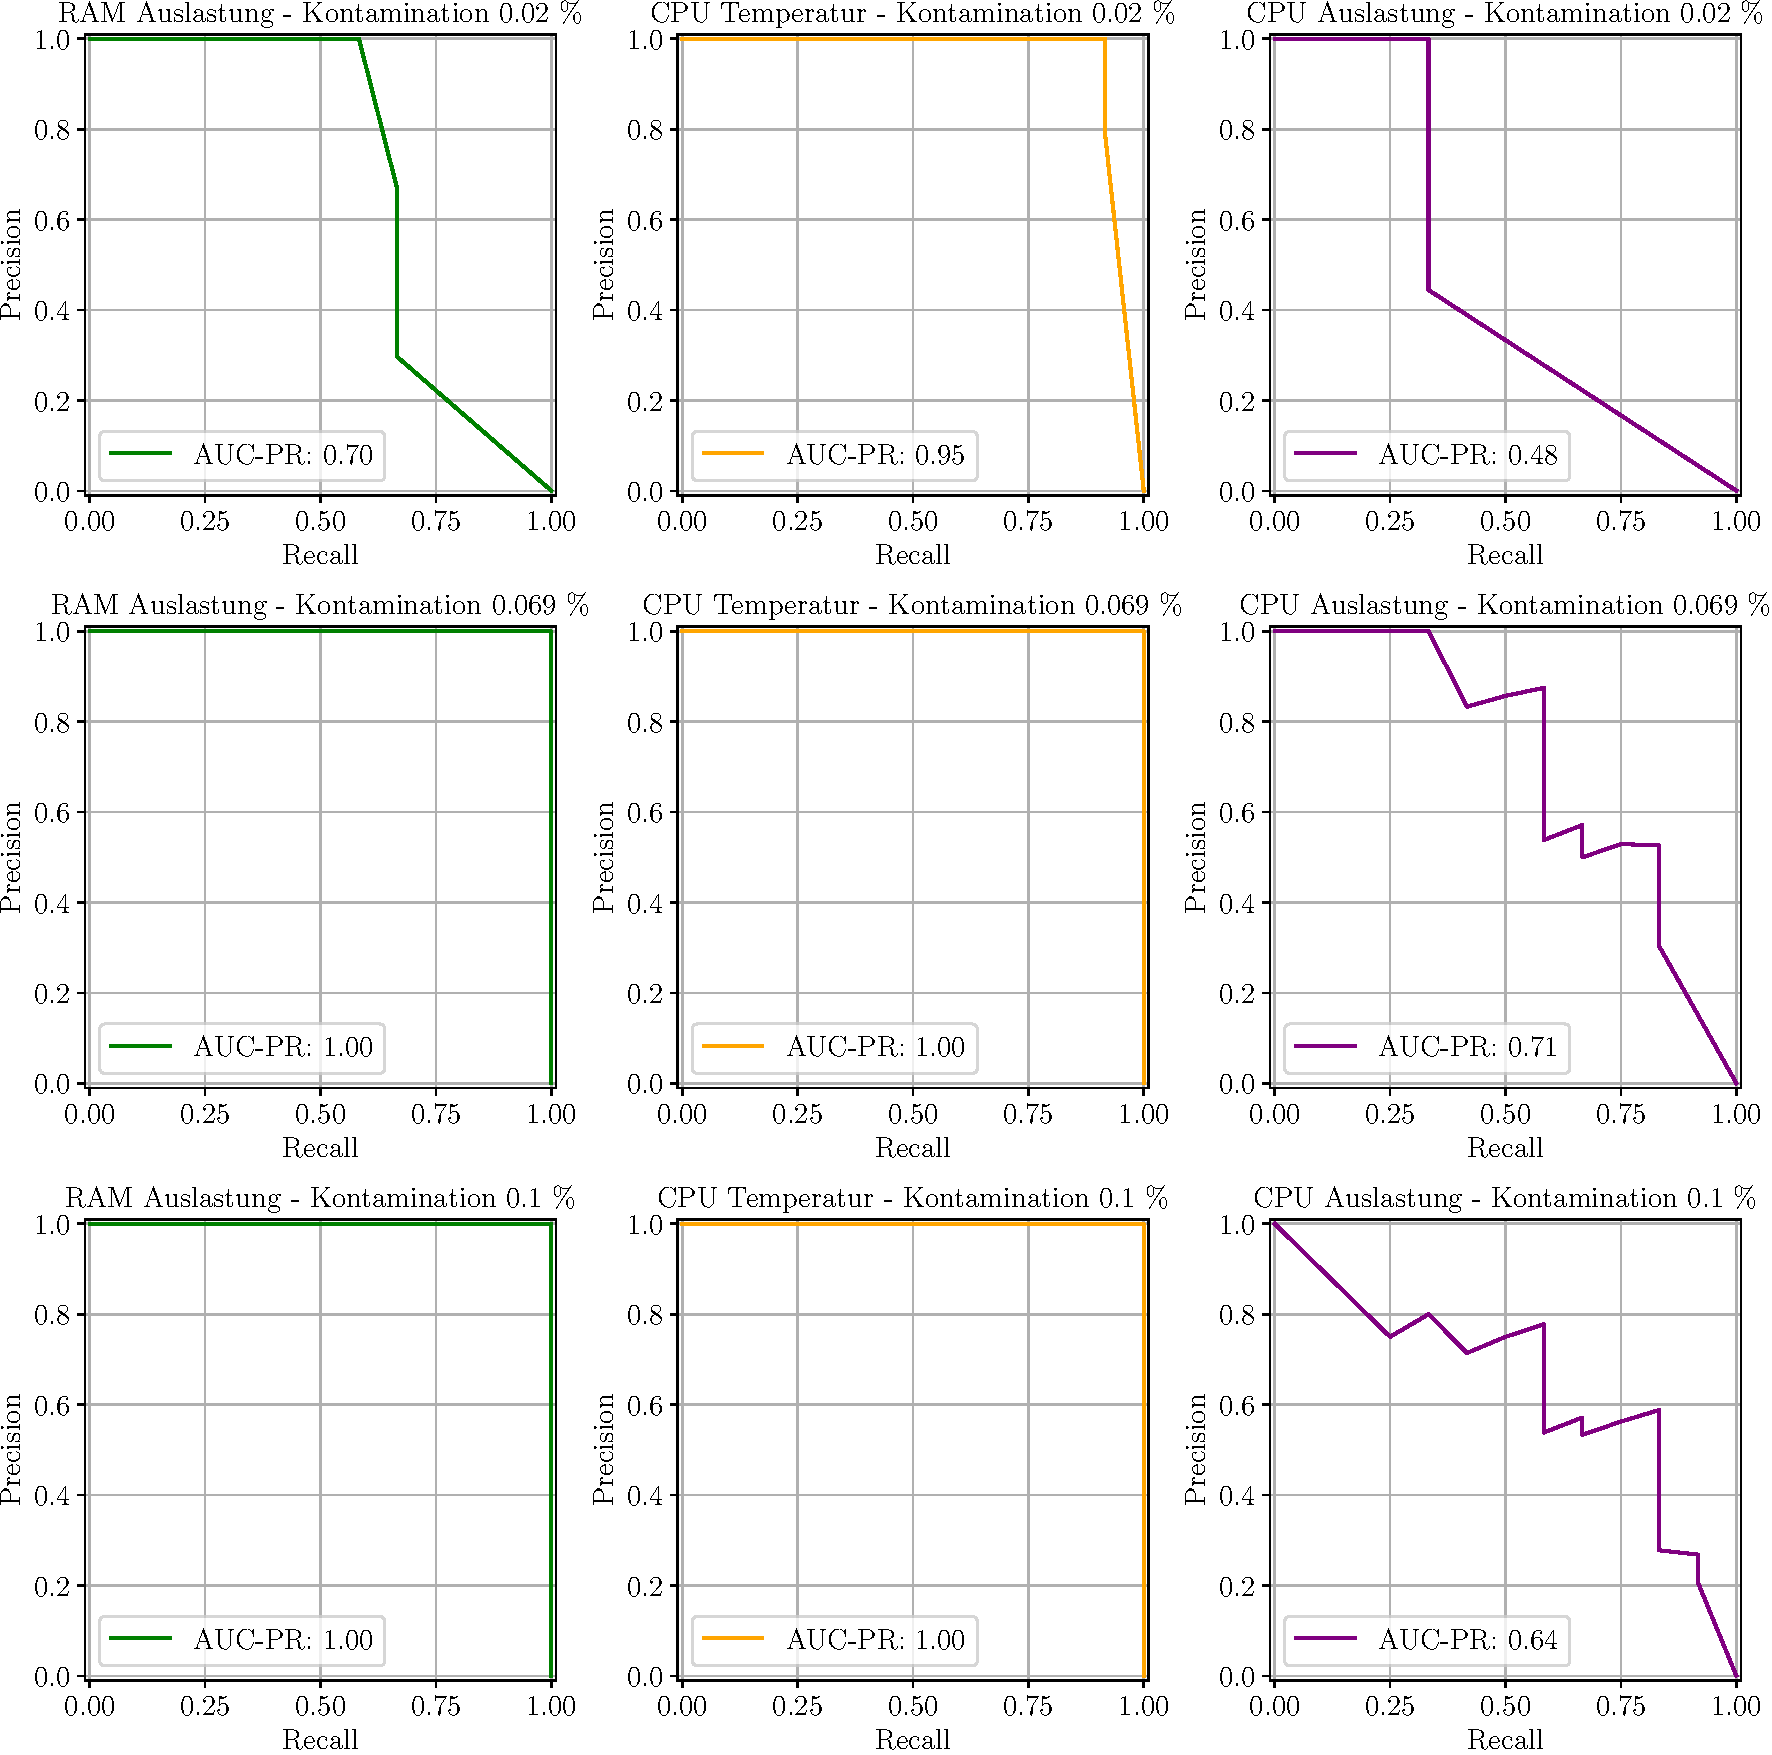
\includegraphics[width=1\linewidth]{ch5_anomalieerkennung/abbildungen/SWZ_AUC_PR.pdf}
    \caption{\centering Sliding Window Z-Score: \acp{prkurve} mit \acs*{aucpr} für alle drei Datensätze und die jeweiligen Kontaminationsparameter}
    \label{fig:hbos_auc_pr}
\end{figure}

\begin{figure}[t!]
    \centering
        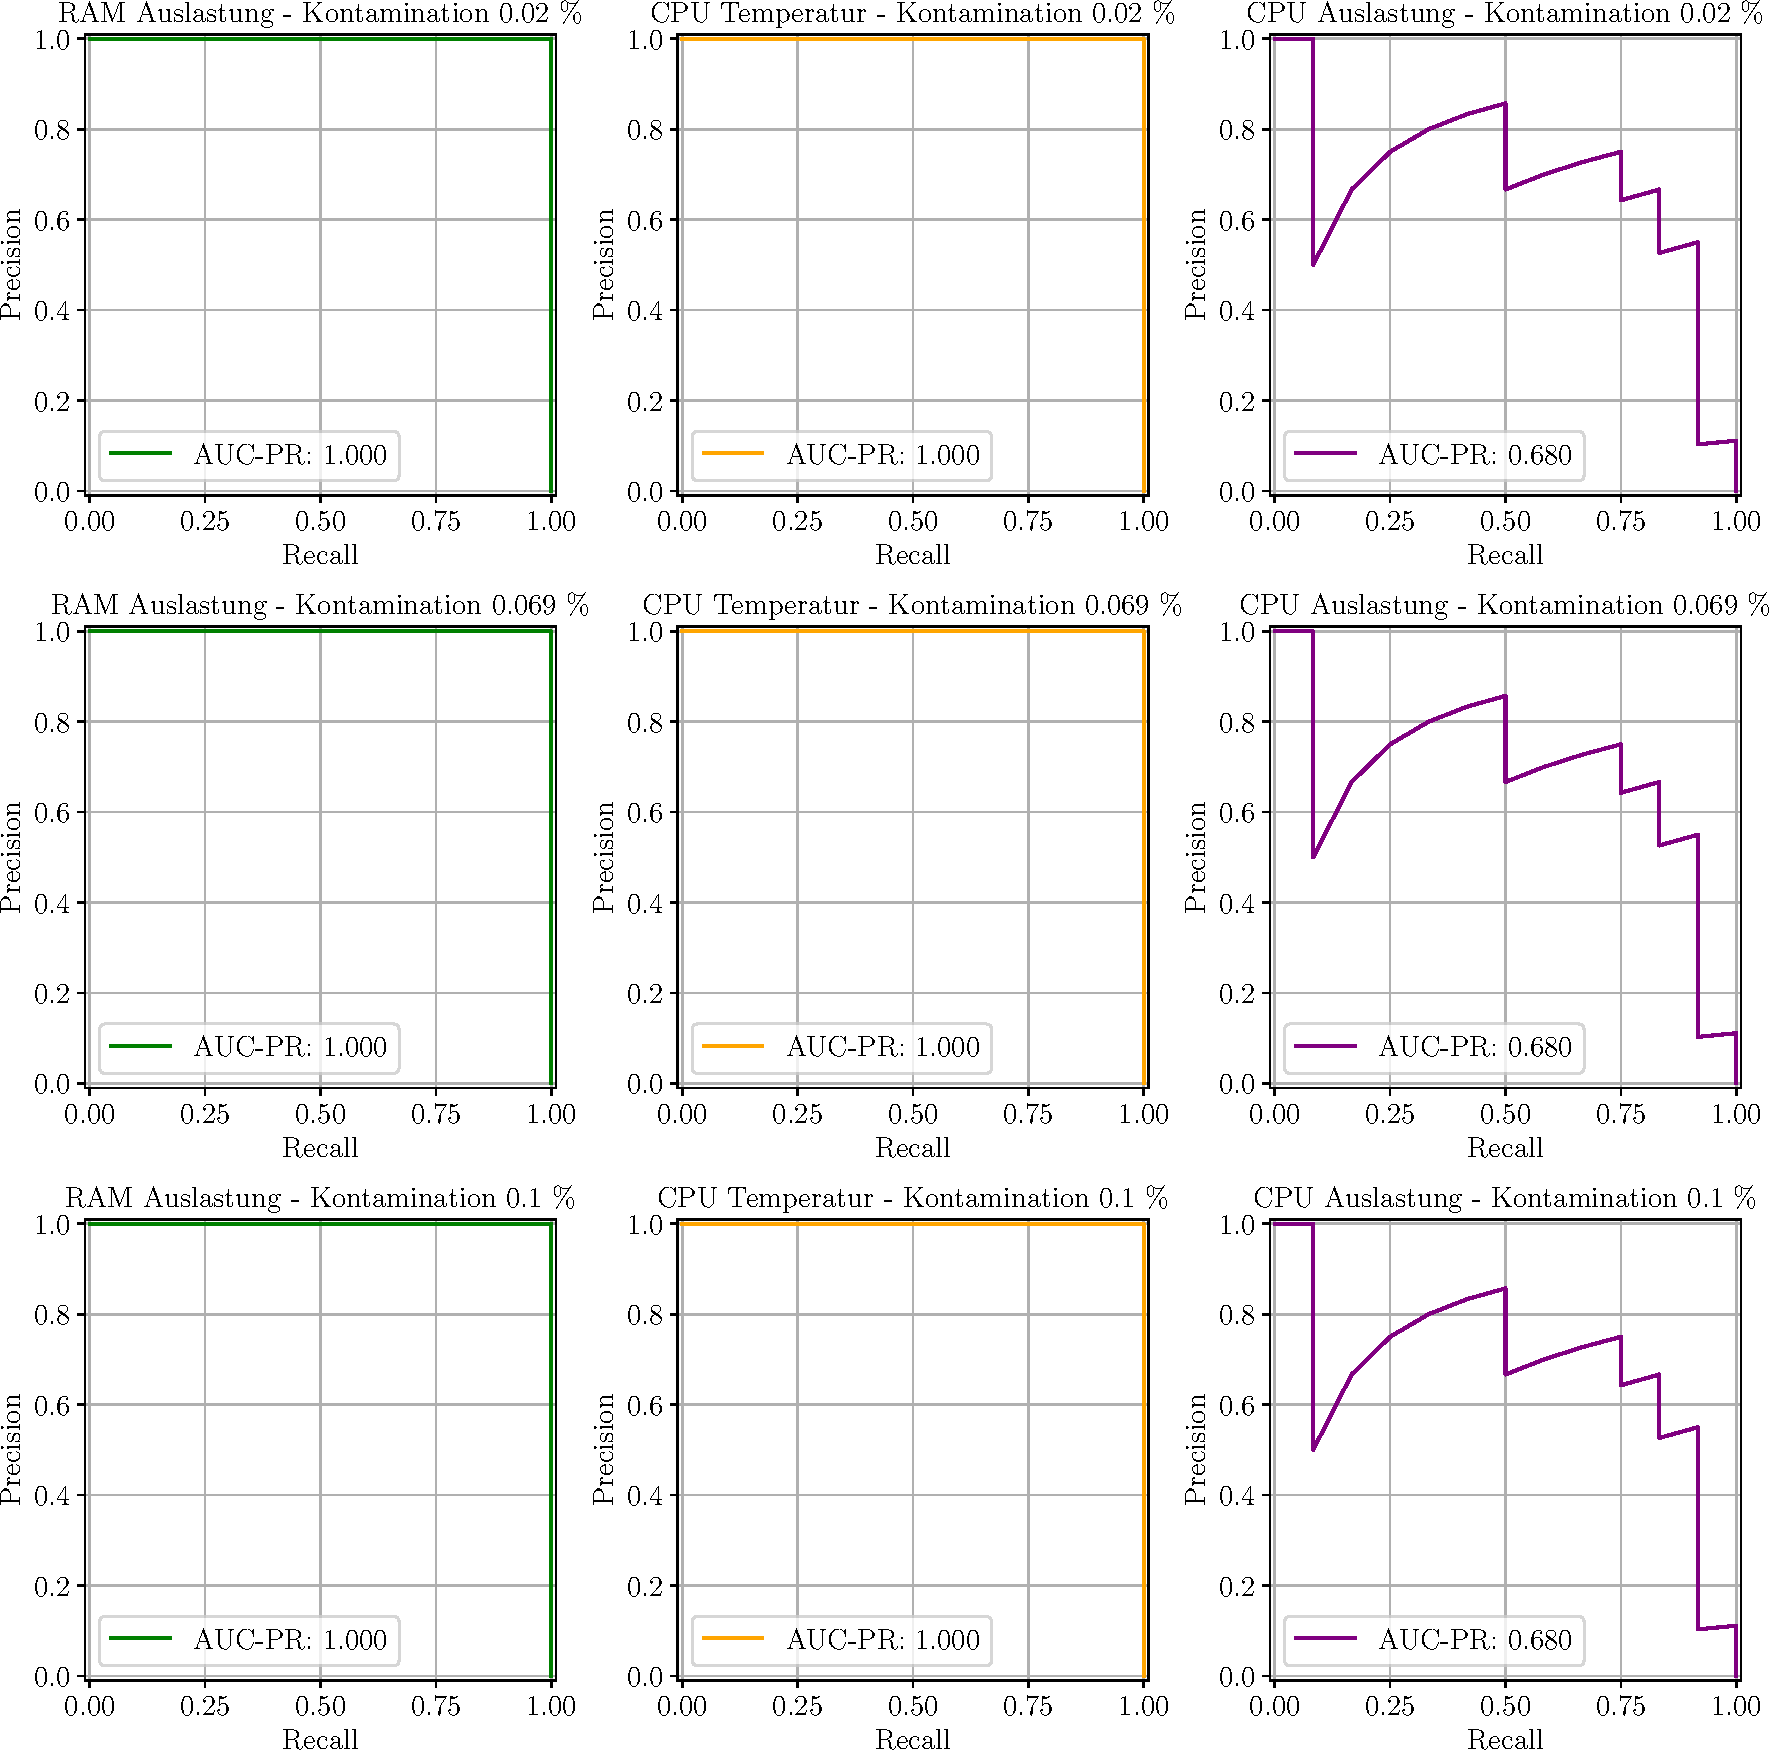
\includegraphics[width=1\linewidth]{ch5_anomalieerkennung/abbildungen/HBOS_AUC_PR.pdf}
    \caption{\centering History Based Outlier Score: \acp{prkurve} mit \acs*{aucpr} für alle drei Datensätze und die jeweiligen Kontaminationsparameter}
    \label{fig:swz_auc_pr}
\end{figure}

Zudem werden mehrere verschiedene Fenstergrößen benutzt, um mögliche Fehlerquellen zu eliminieren. Insgesamt werden 200 verschiedene Fenster
mit Größen zwischen 5 und 1000 Punkten eingesetzt. Für alle drei Kontaminationsparameter kann anhand der \ac{aucpr} die Gesamtperformance des
Algorithmus über mehrere Schwellwerte abgelesen werden. Je höher die \ac{aucpr}, desto besser ist die Performance bzw.~Präzision des Algorithmus
über mehrere Schwellen und demnach weniger abhängig von der Wahl der optimalen Schwelle, die für reale Daten ohnehin schwer zu bestimmen ist.

Die \ac{prkurve} gibt ein gesamtheitliches Bild über einen Algorithmus ab, doch es ist wichtig zu verstehen, wie sich das Bild zusammensetzt. Dazu gibt
\hyperref[fig:auc_pr_beispiel]{Abb.~\Ref*{fig:auc_pr_beispiel}} bereits erste Hinweise. Die zwei Algorithmen schließen ihre Analyse zur Anomaliedetektion
ab, indem eine Sequenz an Anomaliescores zurückgegeben wird. Jeder Index dieser Sequenz korrespondiert genau zum gleichen Index der Eingansgdaten, in dem Fall
die übergebenen Testdatensätze. Der Algorithmus vergibt für jeden Punkt eine Bewertung, die als Anomaliewahrscheinlichkeit interpretiert werden. Je
höher der Wert, desto wahrscheinlich handelt es sich um eine Anomalie. Bei einer perfekten Performance eines Algorithmus erhält jede Anomalie also die
höchste Bewertung, was einer Wahrscheinlichkeit von 100 \% entspricht. Normale Punkte hingegen sollten die niedrigste Bewertung erhalten, also eine
Anomaliewahrscheinlichkeit von 0\%. Für jeden möglichen Schwellwert werden sowohl Precision als auch Recall berechnet und zur \ac{prkurve} zusammengesetzt.
Das heißt jeder Punkt auf der \ac{prkurve} entspricht einem Paar von Precision und Recall eines bestimmten Schwellwerts.
Liegt eine eindeutige Trennung des Algorithmus in der Anomaliebewertung zwischen normalen und anomalen Punkten vor, so drückt sich dies durch einen
hohen \ac{aucpr} Wert aus, während eine undeutlichere Trennung, also normale und anomale Punkte, die jeweils im Bereich zwischen 0 und 100 \% Wahrscheinlichkeit
liegen, dafür sorgen, dass bestimmte Schwellwerte diese Punkte falsch einordnen, und der \ac{aucpr} Wert wird verringert.

Auffällig ist, dass beide Algorithmen nur wenige Probleme mit den beiden Datesätzen zur \ac{ram} Auslastung sowie zur \ac{cpu} Temperatur haben, während
die \ac{cpu} Auslastung bei beiden schlechtere Ergebnisse aufweist. Der Grund liegt in der ungleichmäßigeren Natur der Daten, die innerhalb weniger
Datenpunkte oft Sprünge um mehrere Standardabweichungen verzeichnen. Über alle drei Kontaminationsparameter zeigt sich \ac{hbos} als der robustere
der zwei Algorithmen, da er mit Ausnahme der Testdaten zur \ac{cpu} Auslastung unabhängig jeglicher Parametrisierung ist.

Desweiteren ist zu erwähnen, dass \ac{hbos} gegenüber \ac{swz} eine um ein Vielfaches höhere Rechendauer benötigt. Für die gezeigten Testdatensätze
betrug die Rechendauer für \ac{hbos} 150 Minuten, während \ac{swz} die Analyse in nur 10 Sekunden abschließen konnte.

\section{Detektion von Subsequenzanomalien}
Die herausgearbeiteten Algorithmen zur Detektion von Subsequenzanomalien werden ebenfalls anhand von drei Datensätzen erprobt und evaluiert.
Ähnlich zu~\hyperref[sec:punktanomaliedetektion]{Abs.~\Ref*{sec:punktanomaliedetektion}} werden dazu die \ac{ram} Auslastung sowie die \ac{cpu} Temperatur
herangezogen und um realistische Subsequenzanomalien ergänzt. Desweiteren liegt ein Datensatz zur Stromaufnahme des Blitzmoduls vor.

Als mögliches Anomalieszenario liegt für die \ac{ram} Auslastung ein plötzlicher, linearer Anstieg der Auslastung vor. Im normalen Betriebszustand
ist die Auslastung näherungsweise konstant. Im Datensatz zur \ac{cpu} Temperatur wurden zwei Anomaliefälle hinzugefügt, ein sprungartiger Anstieg
sowie eine starke Schwankung im Positiven wie im Negativen. Beide Fälle entsprechen ebenfalls nicht dem Normalzustand, da die \ac{cpu} Temperatur
in erster Linie von der \ac{cpu} Auslastung abhängt, welche näherungsweise konstant verläuft. Außerdem korreliert die \ac{cpu} Temperatur
mit der Außentemperatur, welche keinen starken Schwankungen innerhalb weniger Stunden ausgesetzt ist, wie sie im vorliegenden Anomaliefall
auftreten. Zuletzt liegen für das Blitzmodul zwei Anomaliefälle vor. Der normale zeitliche Verlauf des Blitzmoduls beschränkt sich auf einen
Ruhestrom von etwa 0,3 A sowie einen kurzen Impuls auf einen Maximalstrom von 3,5 A beim Auslösen des Blitzes. Als anomale Ereignisse liegen
zum einen ein Rippelstrom vor, dessen Problematik sich vor allem auf unerwünschtes EMV-Verhalten bezieht, und ein lang anhaltender Maximalstrom,
der entweder für einen Auslösefehler oder einen Sensordefekt hindeuten könnte. Die ursprünglichen Daten und die ergänzten Anomalien sind in
\hyperref[fig:subsequenz_datensätze]{Abb.~\Ref*{fig:subsequenz_datensätze}} aufgeführt.

\begin{figure}[t!]
    \centering
        \includegraphics[width=1\linewidth]{ch5_anomalieerkennung/abbildungen/subsequenzanomalien_datensätze.pdf}
    \caption{\centering Drei Datensätze, anhand derer die Algorithmen zur Subsequenzanomaliedetektion getestet und evaluiert werden.}
    \label{fig:subsequenz_datensätze}
\end{figure}

Die Evaluierung der Algorithmen erfolgt ebenfalls punktbasiert mithilfe der \ac{prkurve} und \ac{aucpr}, die für \ac{swifd}
in~\hyperref[fig:SWIFD_AUC_PR]{Abb.~\Ref*{fig:SWIFD_AUC_PR}} und für \ac{lstm-ae} in einem ersten Durchlauf
in~\hyperref[fig:LSTMAE_AUC_PR_1]{Abb.~\Ref*{fig:LSTMAE_AUC_PR_1}} vorliegen. Die Untersuchung, und vor allem eine aussagekräftige Evaluierung
mit GrammarViz, gestaltete sich als schwierig, weshalb der Algorithmus bei der Analyse und Gegenüberstellung außen vor bleibt. \ac{lstm-ae} gehört
zur Lernklasse der Semi-Supervised Algorithmen, daher bedarf es Trainingsdaten, bevor eine Anomaliedetektion durchgeführt werden kann.

\begin{figure}[t!]
    \centering
        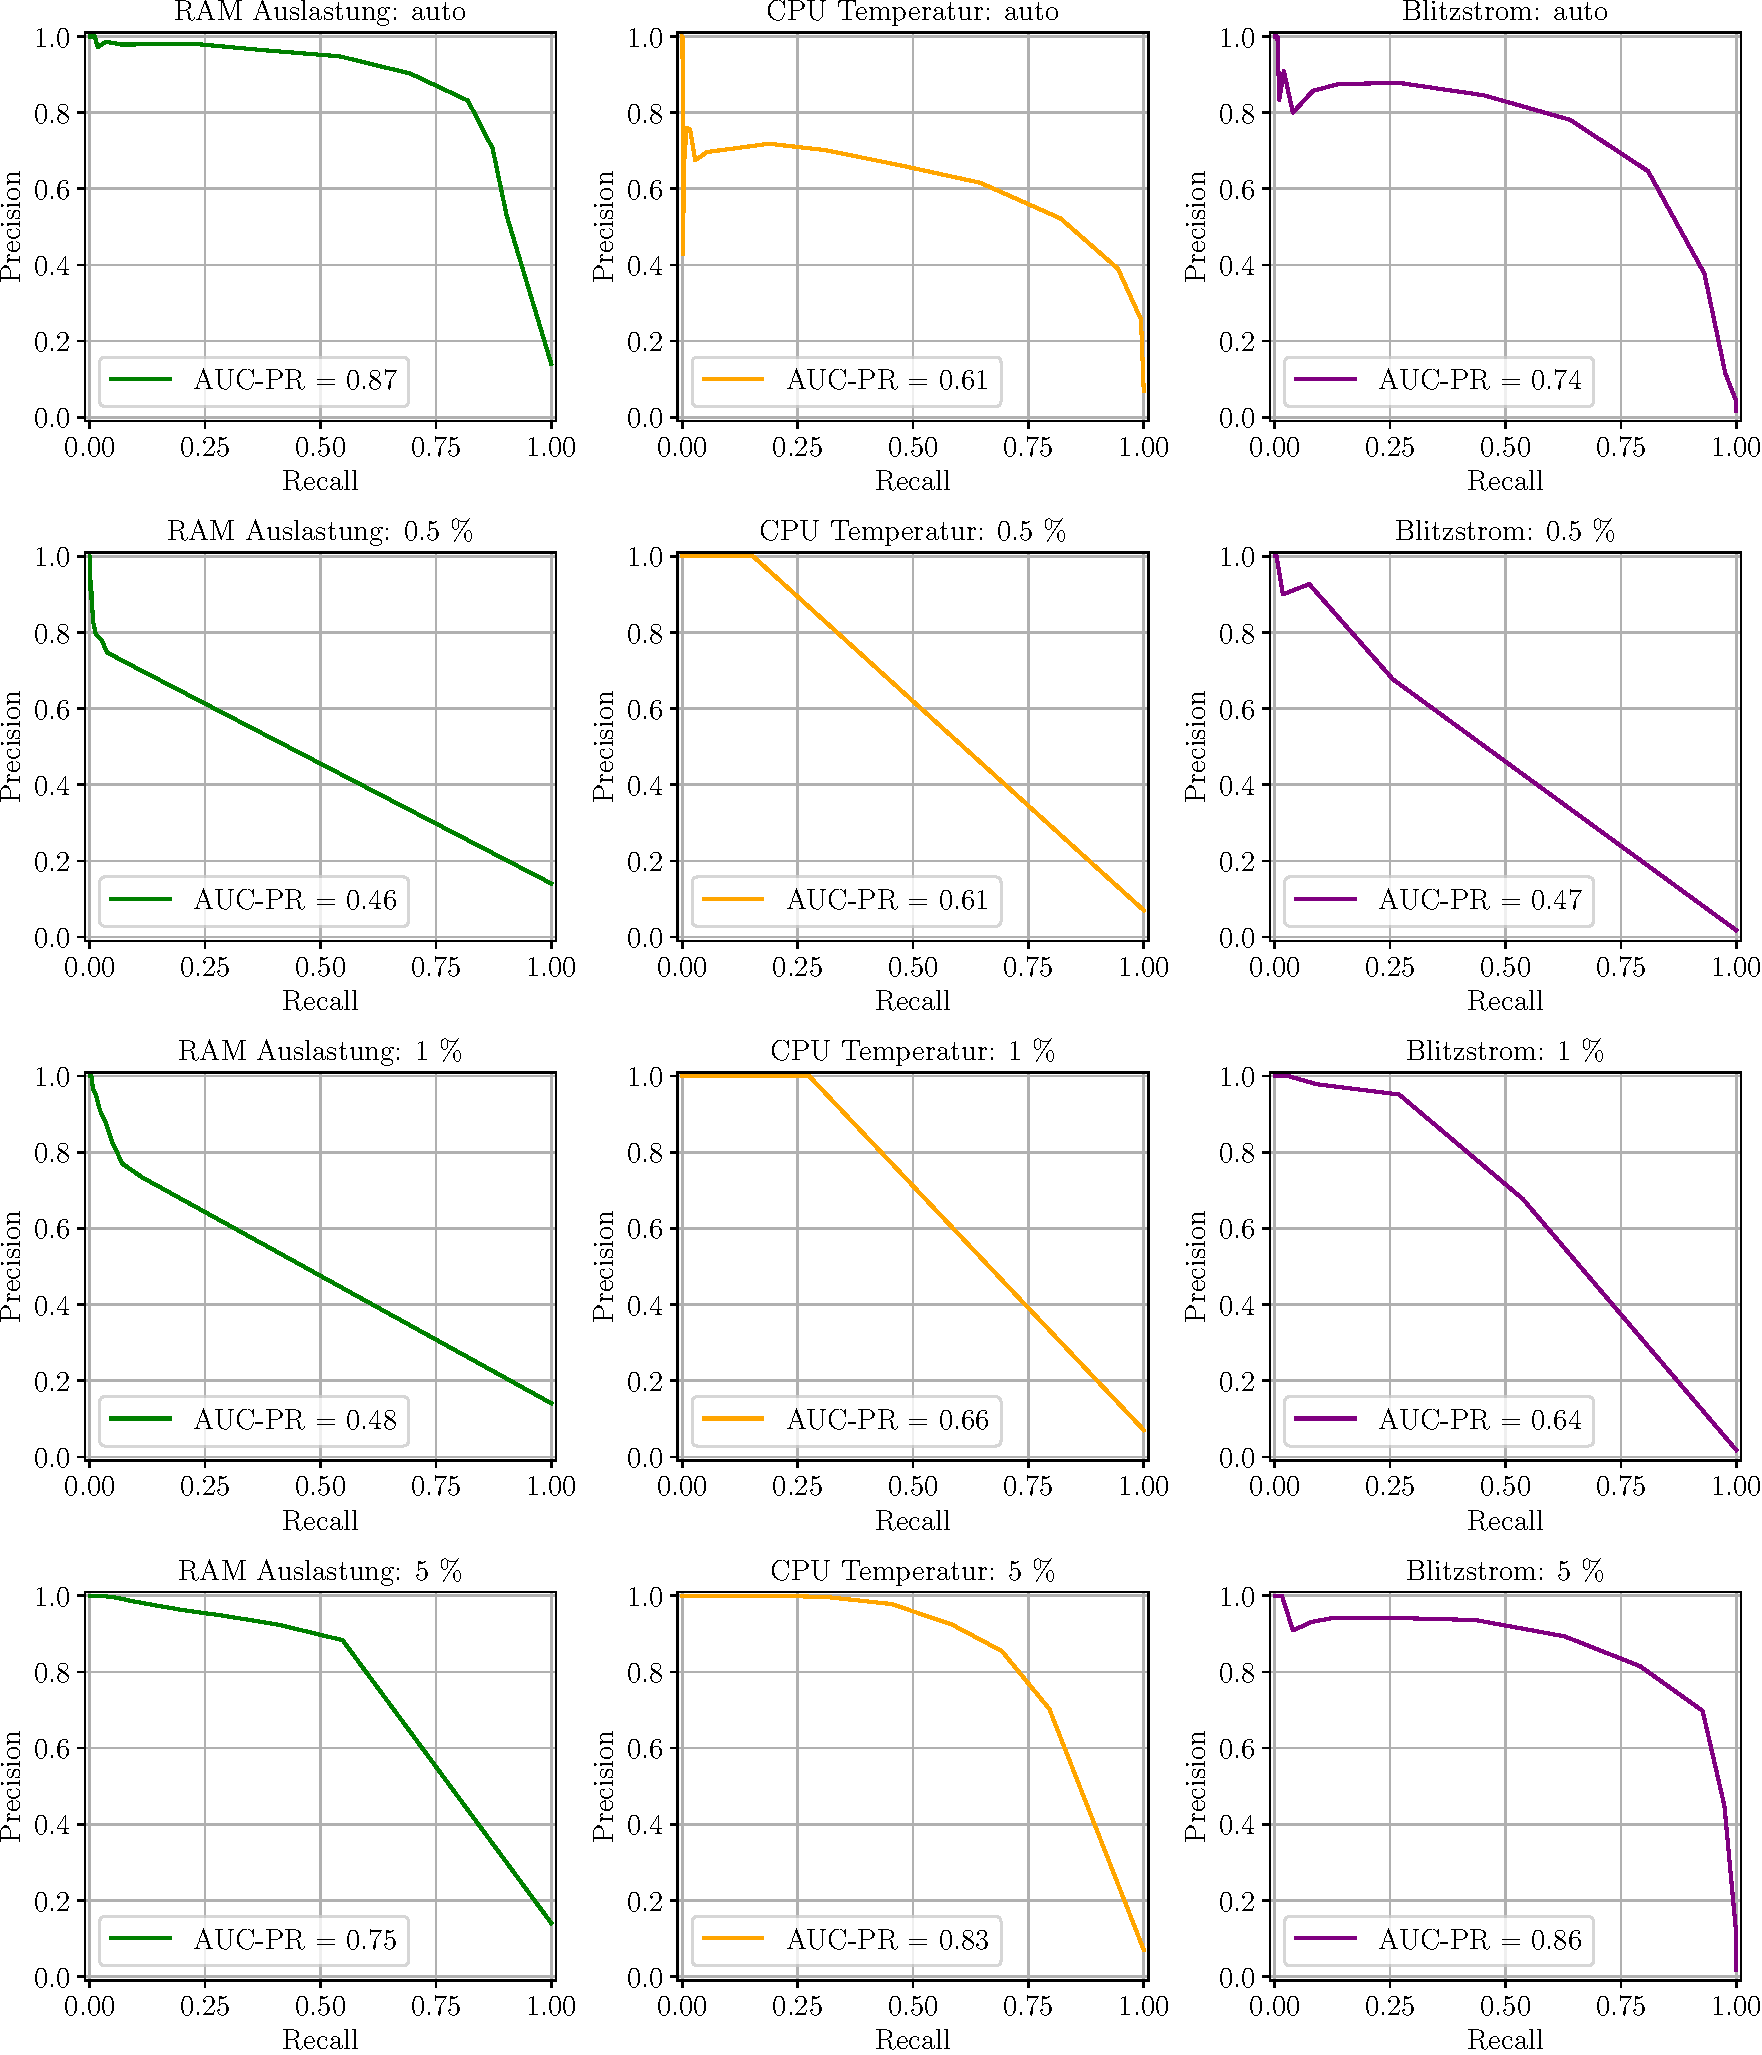
\includegraphics[width=1\linewidth]{ch5_anomalieerkennung/abbildungen/SWIFD_PR_AUC_PR.pdf}
    \caption{\centering \acp{prkurve} inkl.~\acs*{aucpr} für alle Datensätze nach Analyse durch \acs*{swifd} mit vier Kontaminationsparametern:
    automatisch, 0,5 \%, 1 \% und 5 \%.}
    \label{fig:SWIFD_AUC_PR}
\end{figure}

Analog zu~\hyperref[sec:punktanomaliedetektion]{Abs.~\Ref*{sec:punktanomaliedetektion}} werden mehrere Fenster variabler Größe sowie mehrere
Kontaminationsparameter verwendet, um ein weniger an einzelne Parameter gebundenes Ergebnis zu erhalten. Die Gegenüberstellung
beschränkt sich daher allein auf die \acp{prkurve} sowie \ac{aucpr}, da für ein \ac{lstm} keine zusätzlichen Parameter benötigt werden, die mit denen
in \ac{swifd} verglichen werden können. Die Performance des \ac{lstm-ae} hinsichtlich Genauigkeit und Fehlererkennungsrate bzw.~Precision und Recall
ist in aller erster Linie davon abhängig, mit welchen Hyperparametern er trainiert wurde~\cite{Wei2022}~\cite{Lachekhab2024}.

\begin{figure}[t!]
    \centering
        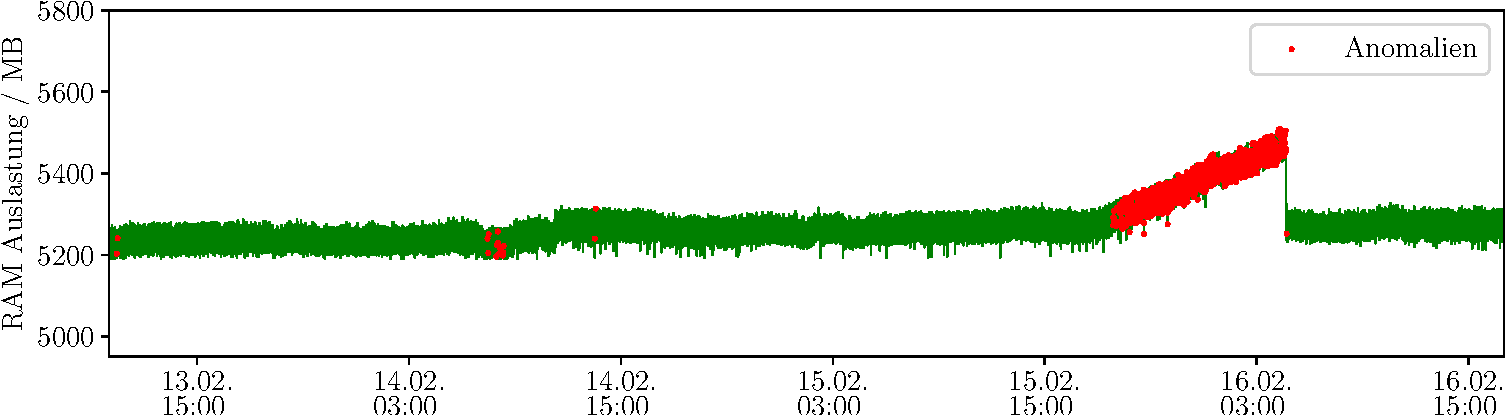
\includegraphics[width=1\linewidth]{ch5_anomalieerkennung/abbildungen/SWIFD_Ergebnis_RAM.pdf}
    \caption{\centering Als Anomalie detektierte Punkte durch \acs*{swifd} werden rot markiert. Der passende Schwellwert für anomale Punkte konnte durch Optimierung
    des F1-Scores in Abhängigkeit von Precision und Recall ermittelt werden}
    \label{fig:SWIFD_visualisierung}
\end{figure}

Durch weiteres Training oder aber die Initialisierung eines neuen Modells veränderter Architektur mit Erweiterung um mehrere \ac{lstm}-Schichten
kann die Performance verbessert werden, sollte sie noch nicht zufriedenstellend sein. Allerdings bedeutet eine komplexere Architektur nicht zwangsläufig
eine genauere Vorhersage oder Detektion. Während das Training in~\hyperref[fig:LSTMAE_AUC_PR_1]{Abb.~\Ref*{fig:LSTMAE_AUC_PR_1}} mit größtenteils
voreingestellten Parametern durchgeführt wurde, so wurden danach weitere Trainings mit neuen Modellen und komplexeren Architekturen durchgeführt,
die aber nicht bei allen Datensätzen zu besseren Ergebnissen führen, wie~\hyperref[fig:LSTMAE_AUC_PR_2]{Abb.~\Ref*{fig:LSTMAE_AUC_PR_2}} zeigt.

Auch die Evaluierung anhand verschiedener Metriken ist nur insoweit aussagekräftig, wie es die Qualität der Testdaten zulässt. Es liegt in der Natur
der Sache, dass reale Daten, auch wenn sie synthetisch um bestimmte Anomalien erweitert wurden, Schwankungen unterliegen, die vom menschlichen Auge
als normal eingestuft werden. Ein Algorithmus hingegen vermag ein ungewöhnliches Muster finden und es als solches markieren, und damit sein eigenes
Testergebnis verschlechtern.

\begin{figure}[b!]
    \centering
        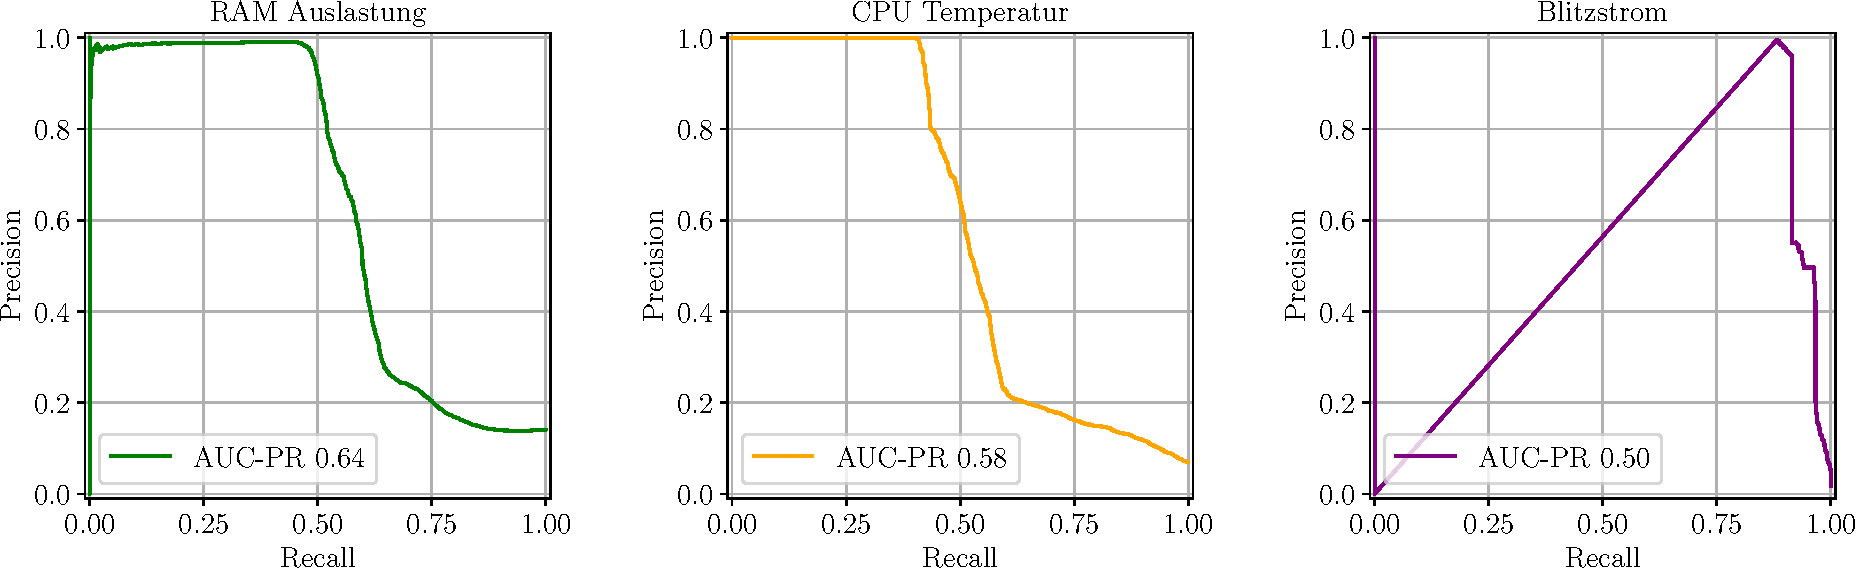
\includegraphics[width=1\linewidth]{ch5_anomalieerkennung/abbildungen/LSTMAE_PR_AUC_PR_1.pdf}
    \caption{\centering \acp*{prkurve} und \acs*{aucpr} für das \acs*{lstm-ae} Modell mit Default Parametern ohne Feintuning}
    \label{fig:LSTMAE_AUC_PR_1}
\end{figure}

\begin{figure}[b!]
    \centering
        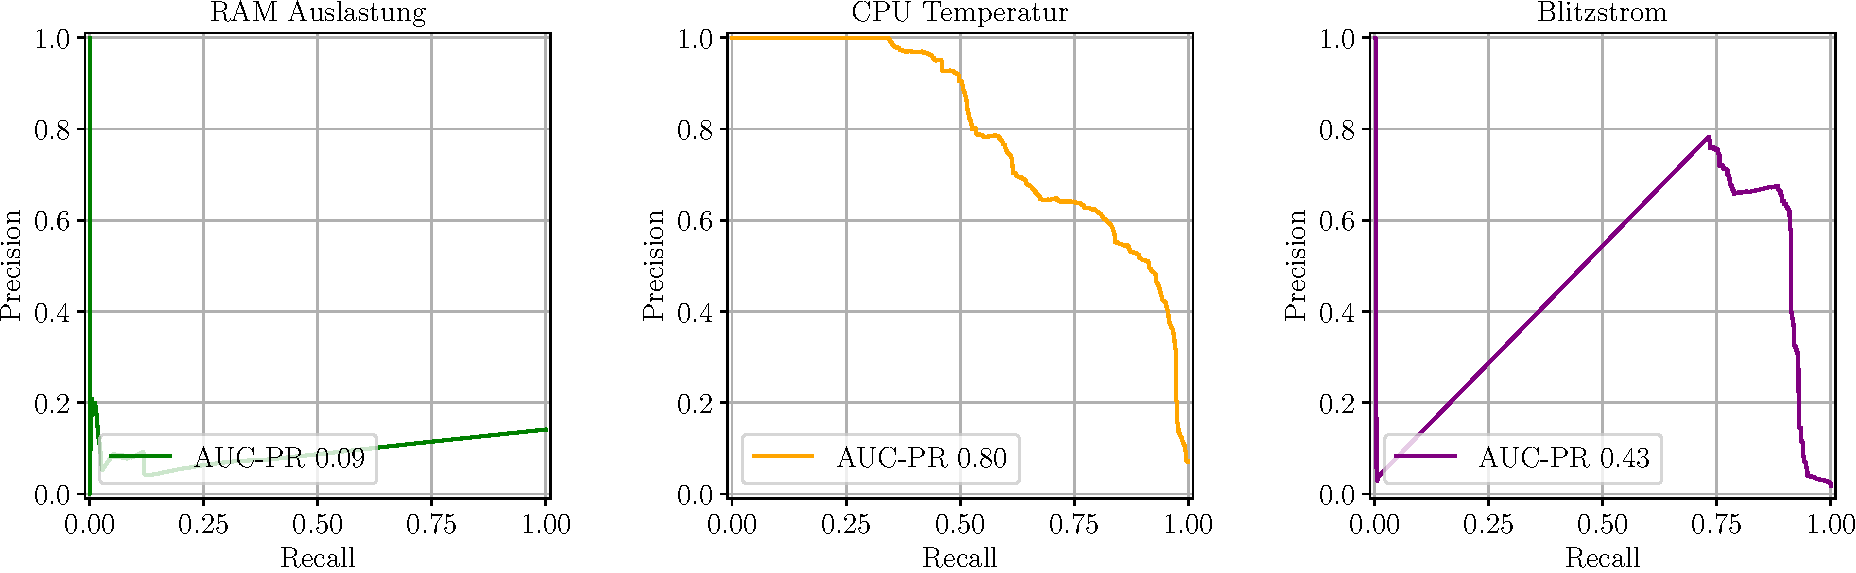
\includegraphics[width=1\linewidth]{ch5_anomalieerkennung/abbildungen/LSTMAE_PR_AUC_PR_2.pdf}
    \caption{\centering \acp*{prkurve} und \acs*{aucpr} für das \acs*{lstm-ae} Modell mit weiter angepassten Parametern wie einer erhöhten Batchgröße und mehr Epochen
    im Training.}
    \label{fig:LSTMAE_AUC_PR_2}
\end{figure}

Eine Ursache dafür, dass ein Algorithmus keine genauen Vorhersagen treffen kann, kann auch ein noch nicht passendes Verhältnis von Trainingsdaten zu
Testdaten sein. Pauschale Annahmen, um Modelle für unterschiedliche Datensätze gleich zu trainieren, sind also offensichtlich keine zuverlässige
Herangehensweise. Hyperparameter Tuning ist ein entscheidender Schritt zur Optimierung von Machine Learning Modellen wie dem \ac{lstm-ae}, da es direkte
Auswirkungen auf die Modellleistung hat. Methoden wie Grid Search, Random Search oder Bayessche Optimierung helfen dabei, optimale Parameter zu finden,
allerdings sind sie oft rechenintensiv und erfordern große Datenmengen. Eine Herausforderung besteht darin, dass übermäßig komplexe Modelle nicht immer
zu besseren Ergebnissen führen und ein Trade-Off zwischen Overfitting und Generalisierung gefunden werden muss~\cite{Iravani2022}.

Die Visualierung der Anomaliedetektion mit \ac{swifd} ist in~\hyperref[fig:SWIFD_visualisierung]{Abb.~\Ref*{fig:SWIFD_visualisierung}} dargestellt. Bei
der Berechnung der Precision-Recall-Kurve kann auch eine optimale Schwelle bestimmt werden, die den höchsten F1-Score zurückgibt. Der F1-Score
leitet sich gem.~\hyperref[eq:fbeta]{Gl.~\Ref*{eq:fbeta}} als $F_\beta$-Score mit $\beta=1$ ab und ist eine weitere Metrik für die Performance eines Algorithmus,
allerdings begrenzt auf einen festen Schwellwert.
\newpage

\section{Detektion von Korrelationsanomalien}

Zuletzt gilt es der Untersuchung der Algorithmen zur Korrelationsanomaliedetektion. Dazu werden drei Testdatensätze verwendet, wie sie
in~\hyperref[fig:korrelationsanomalie_datensätze]{Abb.~\Ref*{fig:korrelationsanomalie_datensätze}} dargestellt sind, mit unterschiedlichen
Szenarien, die alle eine mögliche Anomalie abbilden sollen. Die erste Anomalie beschreibt eine Verletzung der Korrelation zwischen der
\ac{cpu} Last und \ac{cpu} Temperatur, da die \ac{cpu} Temperatur linear steigt, während die \ac{cpu} Last nicht im gleichen Maß zunimmt, sondern tendenziell abnimmt.
Der zweite Fall verletzt die Korrelation zwischen der \ac{cpu} und der Temperatur der Systemplatine~-~\ac{soc}, da sich diese im
Normalfall im Gleichschritt bewegen. Im vorliegenden Fall bleibt die \ac{soc} Temperatur für eine bestimmte Zeitspanne jedoch konstant, während die
\ac{cpu} Temperatur ansteigt und wieder fällt. Auch der dritte abgebildete Fall stellt eine Korrelationsanomalie dar, da im selben Zeitraum die
\ac{soc} Temperatur zwar ebenfalls steigt und fällt, jedoch, im Unterschied zu allen anderen Punkten im Zeitverlauf, zeitlich versetzt.

\begin{figure}[b!]
    \centering
     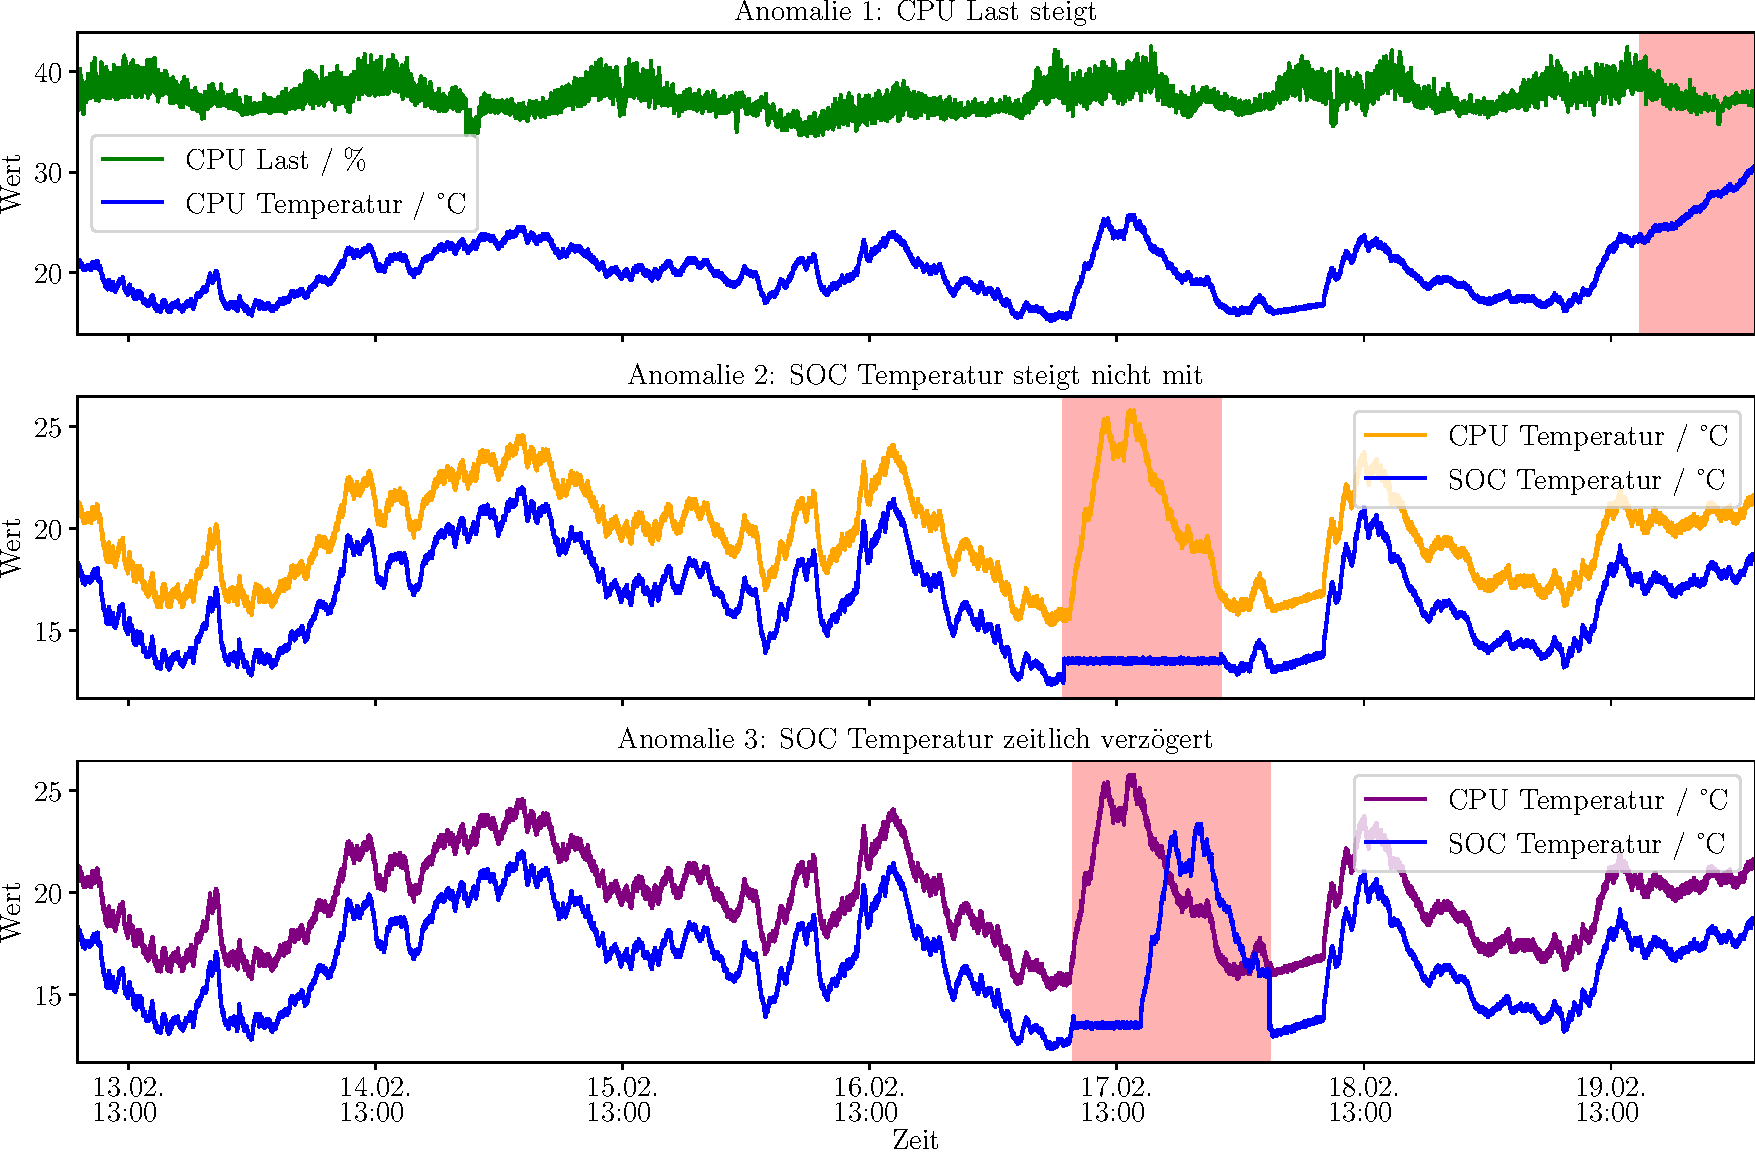
\includegraphics[width=1\linewidth]{ch5_anomalieerkennung/abbildungen/korrealtionsanomalien_daten.pdf}
    \caption{Testdatensätze mit jeweils einer Korrelationsanomalie zwischen zwei Kanälen}
    \label{fig:korrelationsanomalie_datensätze}
\end{figure}

Die untersuchten Algorithmen sind die aus~\hyperref[sec:algorithmen]{Abs.~\Ref*{sec:algorithmen}} für Korrelationsanomalien benannten \ac{md-swifd} und Elliptic
Envelope. Während \ac{md-swifd} noch mit gleitenden Fenstern arbeitet und ebenfalls, wie \ac{hbos}, \ac{swz} und \ac{swifd} auch mit mehreren Fenstergrößen getestet und
ausgewertet wird, benötigt Elliptic Envelope nur einen Parameter zur Angabe der erwarteten Kontamination, der für beide Algorithmen gleich übergeben wird.
Im direkten Vergleich kann Elliptic Envelope über alle Datensätze hinweg höhere \ac{aucpr} Werte  sowie eine gänzliche Unabhängigkeit vom übergebenen
Kontaminationsparameter vorweisen. Das macht den Algorithmus wesentlich robuster im Umgang mit verschiedensten Datensätzen.

\begin{figure}[t!]
    \centering
        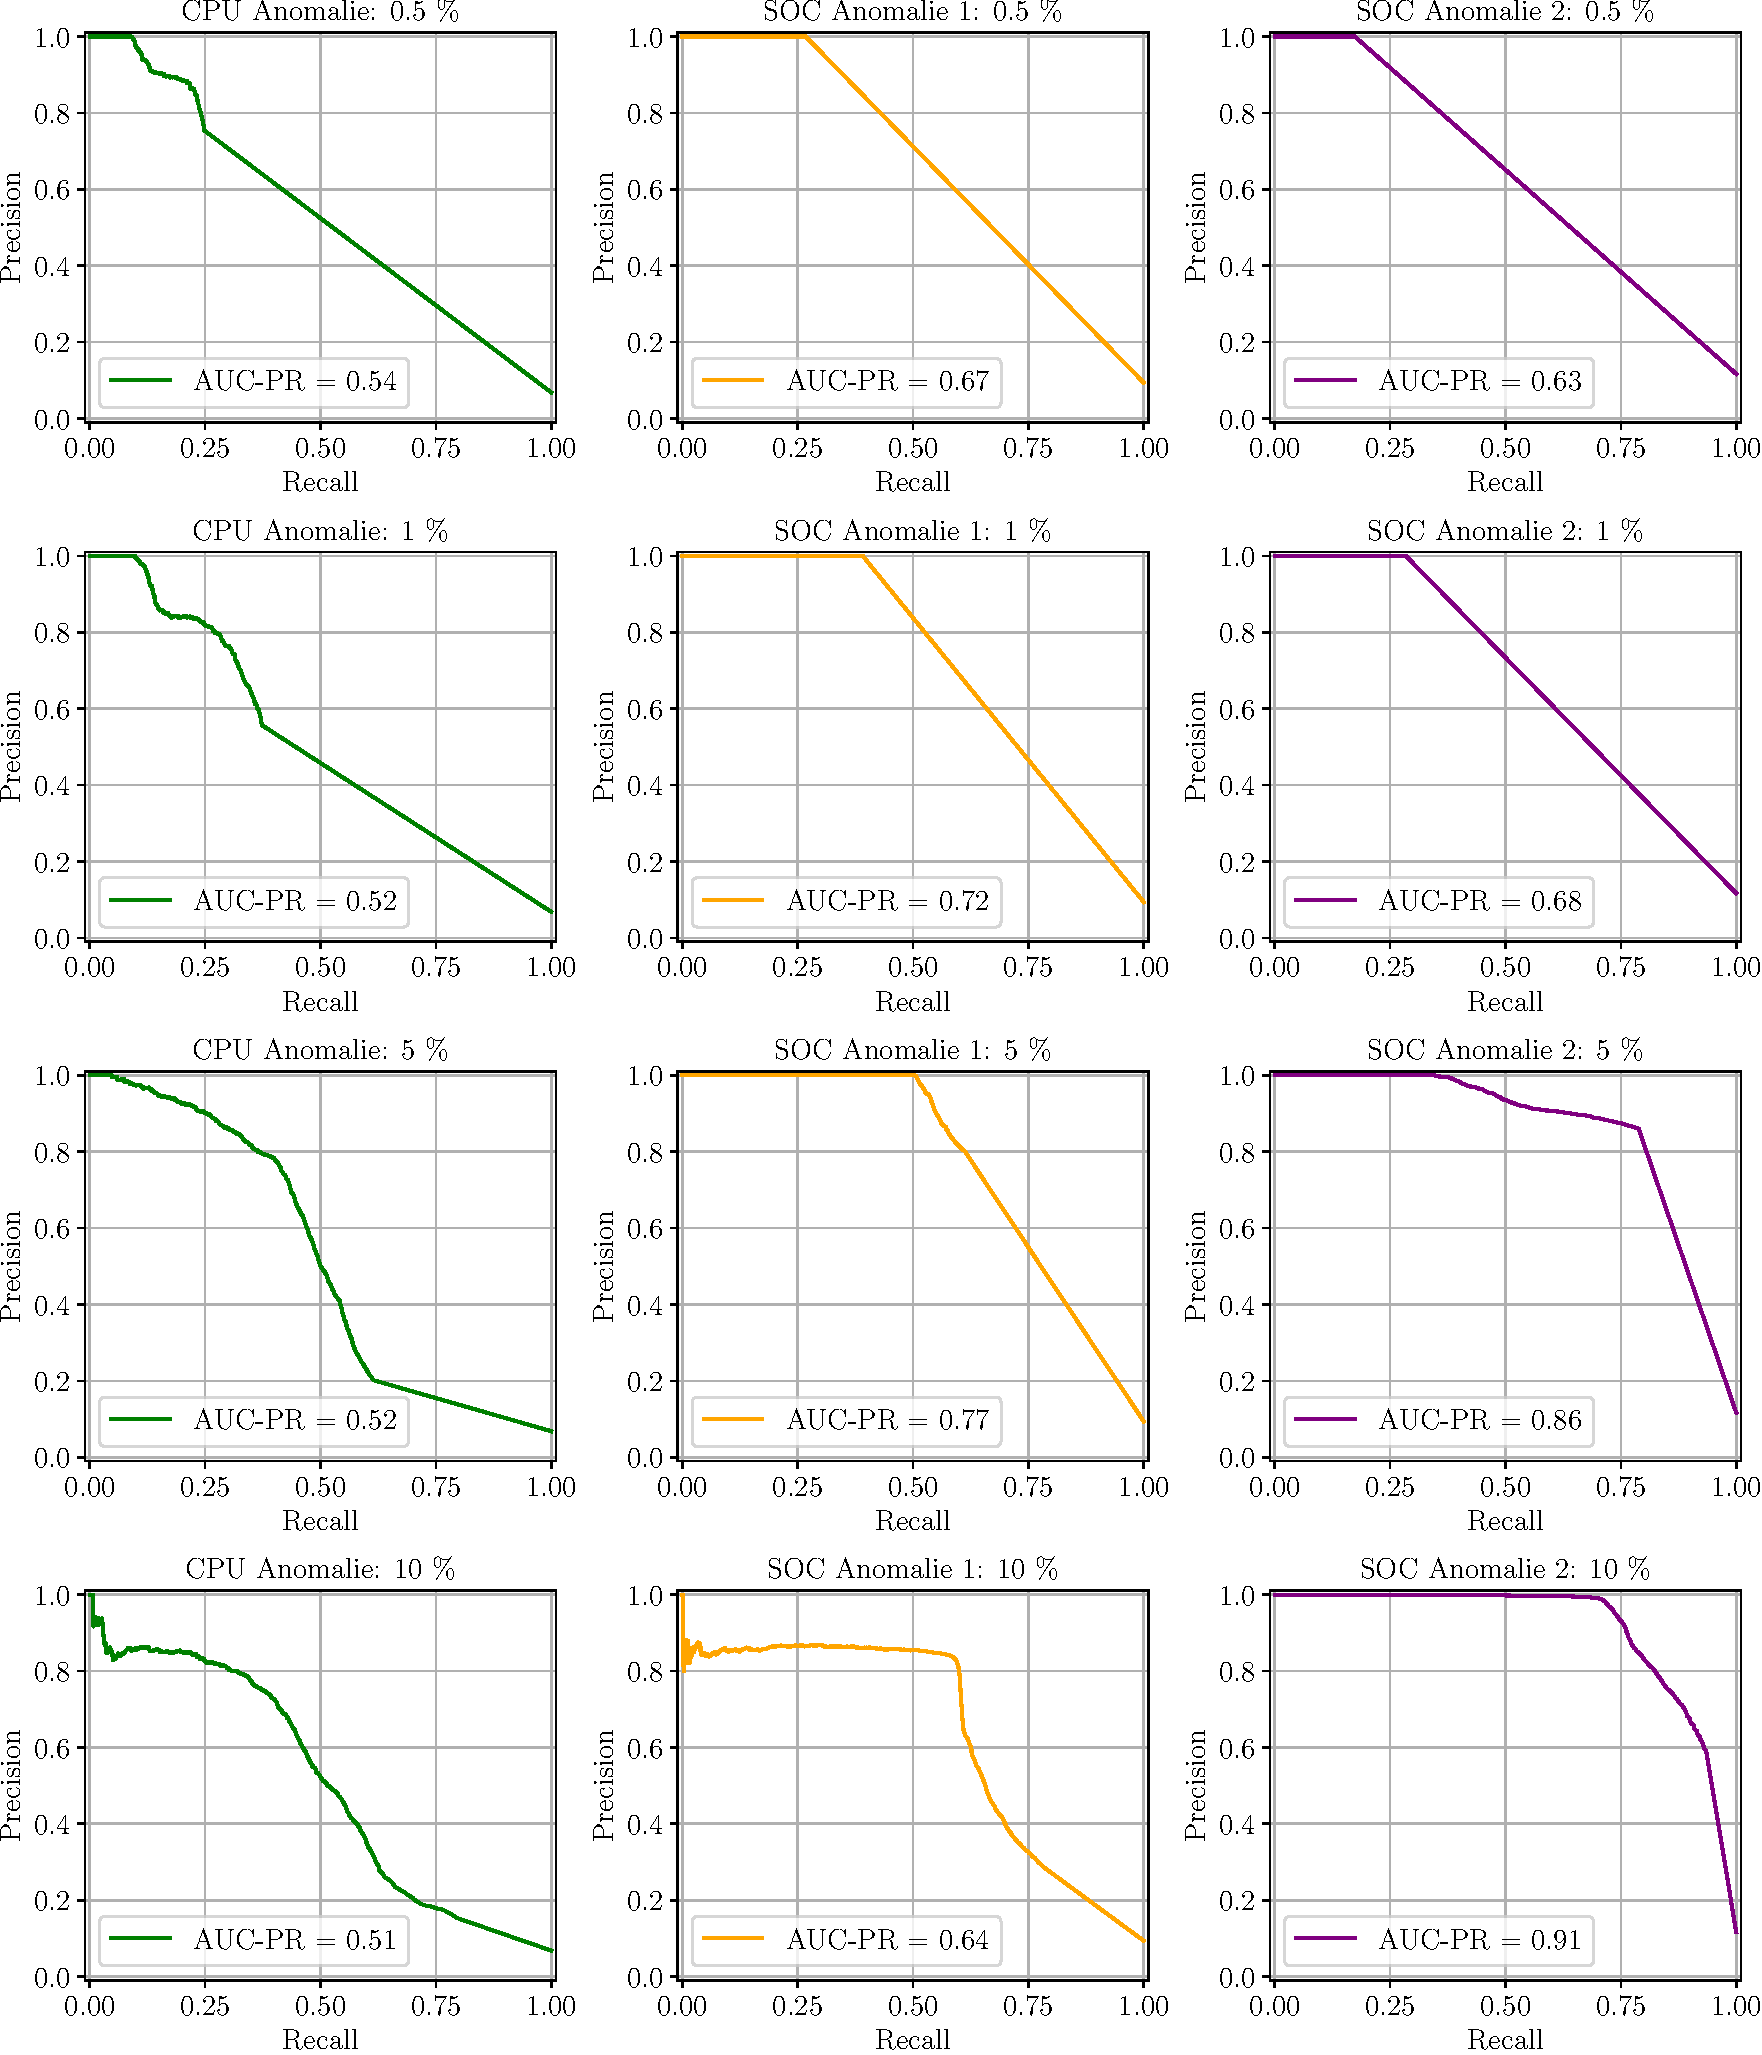
\includegraphics[width=1\linewidth]{ch5_anomalieerkennung/abbildungen/MDSWIFD_PR_AUC_PR.pdf}
    \caption{\centering \acp*{prkurve} und \acs*{aucpr} nach der Anomaliedetektion mit \acs*{md-swifd}. Auch hier sind die Durchläufe mit den vier
    Kontaminationsparametern 0,5 \%, 1 \%, 5 \% und 10 \% dargestellt.}
    \label{fig:MDSWIFD_AUC_PR}
\end{figure}

\begin{figure}[t!]
    \centering
        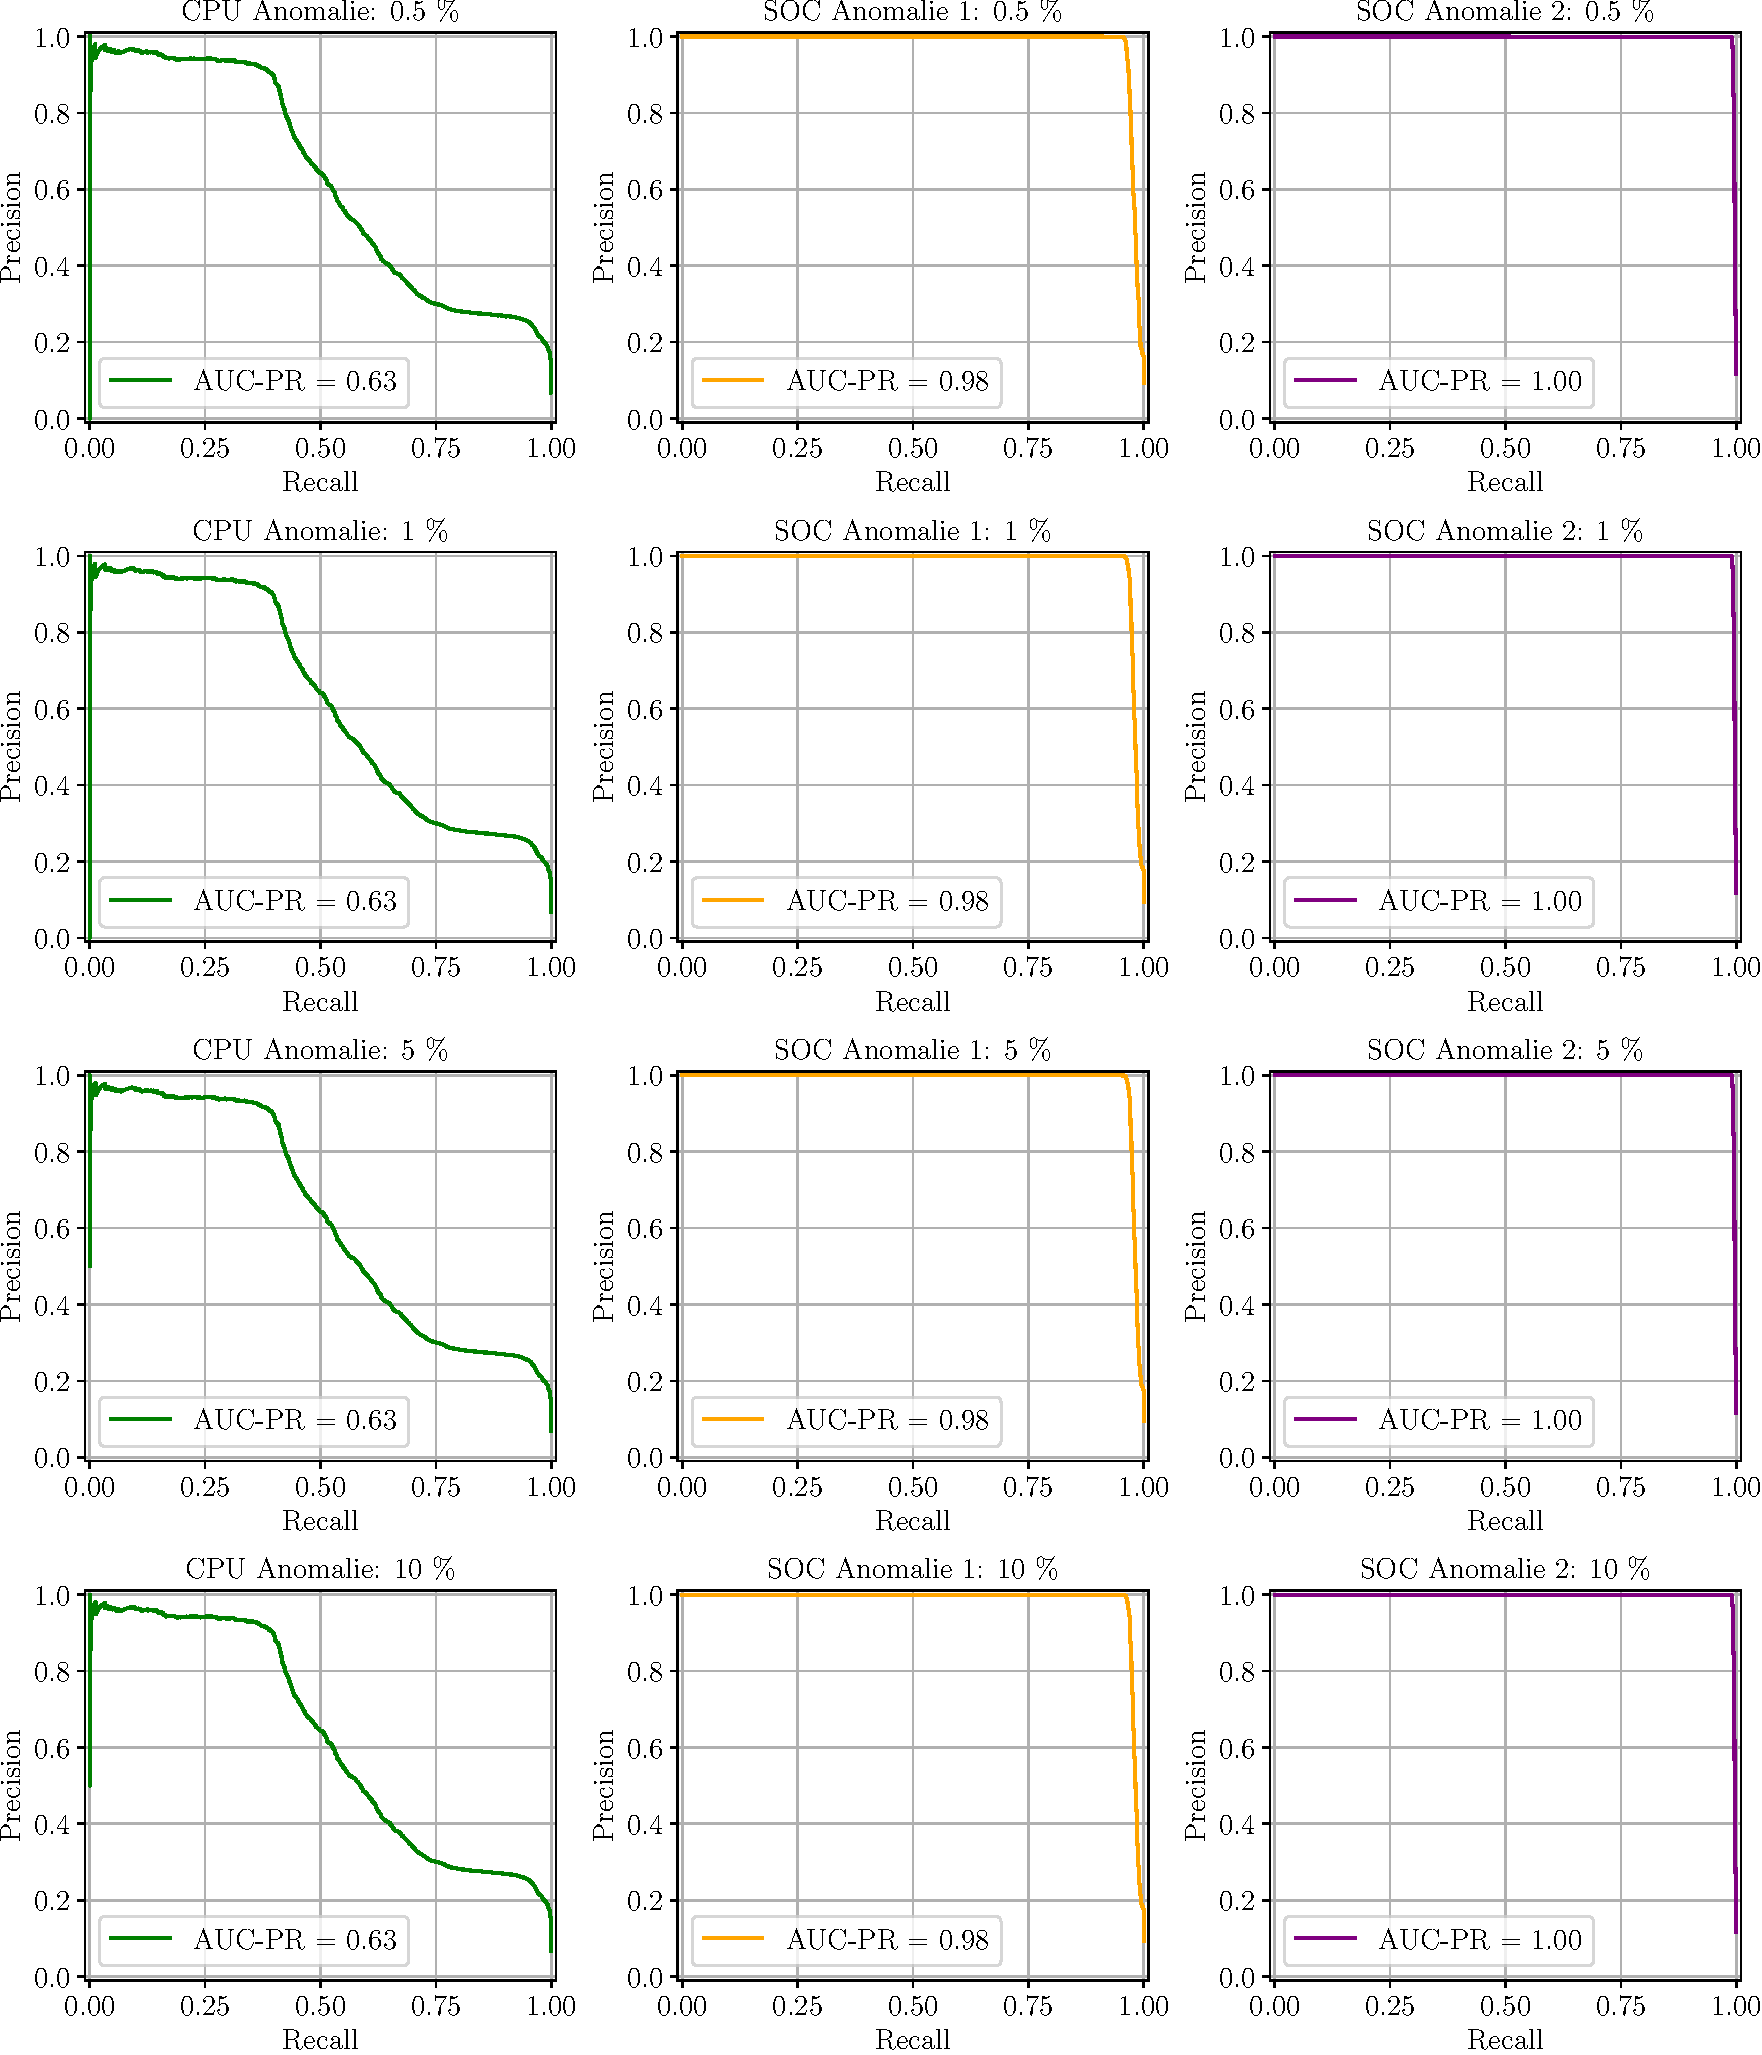
\includegraphics[width=1\linewidth]{ch5_anomalieerkennung/abbildungen/EE_PR_AUC_PR.pdf}
    \caption{\centering \acp*{prkurve} und \acs*{aucpr} nach der Anomaliedetektion mit Elliptic Envelope. Auch hier sind die Durchläufe mit den vier
    Kontaminationsparametern 0,5 \%, 1 \%, 5 \% und 10 \% dargestellt.}
    \label{fig:EE_AUC_PR}
\end{figure}

Wie bereits bei den Ergebnissen der Subsequenzanomaliedetektion erwähnt, ist ein Testergebnis nur so aussagekräftig, wie es die Testdaten erlauben. Während
Korrelationsanomalien eindeutiger feststellbar sind als Subsequenzanomalien, wie die Ergebnisse in~\hyperref[fig:MDSWIFD_AUC_PR]{Abb.~\Ref*{fig:MDSWIFD_AUC_PR}}
und~\Ref{fig:EE_AUC_PR} zeigen, bleibt trotzdem offen, ab wann eine Korrelation wirklich
und merklich verletzt ist. Besonders Anomalie 1 wird sowohl von \ac{md-swifd} in~\hyperref[fig:MDSWIFD_AUC_PR]{Abb.~\Ref*{fig:MDSWIFD_AUC_PR}} als auch von Elliptic
Envelope in~\hyperref[fig:EE_AUC_PR]{Abb.~\Ref*{fig:EE_AUC_PR}} mit geringerer Genauigkeit erkannt als die anderen beiden Anomalien. Die beiden dargestellten
Variablen zur \ac{cpu} Last und Temperatur sind keineswegs perfekt korreliert, aber das Verhalten der einen Größe beeinflusst zweifelsfrei das Verhalten der anderen
Größe. Aber ab wann ist eine Abweichung von diesem Verhalten groß genug, um anomal zu sein? Der eingefärbte rote Bereich kann als Maßstab herangezogen werden, denn er
zeigt die Indizes, die manipuliert wurden, um die Anomalie zu erzeugen. Jedoch entspricht dieser nicht unbedingt der absoluten Wahrheit und beeinflusst trotzdem
die Ergebnisse beider Algorithmen, da \ac{aucpr} für beide Algorithmen geringer ist als bei den anderen beiden Testdatensätzen. Die generelle Funktionalität der beiden
Algorithmen kann also anhand der beiden letzteren Anomalien, die \ac{soc} Temperatur betreffend, nachgewiesen werden. Das schlechtere Ergebnis der Untersuchung der
\ac{cpu} Last Anomalie in Fall 1 soll diesen Eindruck trotzdem nicht abwerten.

Auch für Elliptic Envelope soll das Ergebnis der Anomaliedetektion einmal visualisiert werden, diesmal anhand von Anomalie 3
aus~\hyperref[fig:subsequenz_datensätze]{Abb.~\Ref*{fig:subsequenz_datensätze}}. Hier wurde der optimale Schwellwert ebenfalls anhand der Ergebnisse aus der Berechnung
für Precision und Recall ermittelt. Der Algorithmus ist durch ein sehr robustes Scoring in der Lage, zwischen Normal und Anomalie zuverlässig zu differenzieren.
Von robustem Scoring wird gesprochen, wenn normale Punkte einen sehr niedrigen Anomaliescore nahe dem Minimum erhalten, während Anomalien einen sehr hohen Score
nahe dem Maximum erhalten. Diese klare Differenzierung ist auch den \acp{prkurve} in~\hyperref[fig:EE_AUC_PR]{Abb.~\Ref*{fig:EE_AUC_PR}} zu entnehmen. Das hat zur Folge,
dass eine genaue und präzise Anomaliedetektion nicht davon abhängt, ob genau der optimale Schwellwert zur Auswertung gewählt wird. Der hohe \ac{aucpr} Wert drückt dies
in einem Maß aus, das sich direkt mit \ac{md-swifd} vergleichen lässt.

\begin{figure}[H]
    \centering
        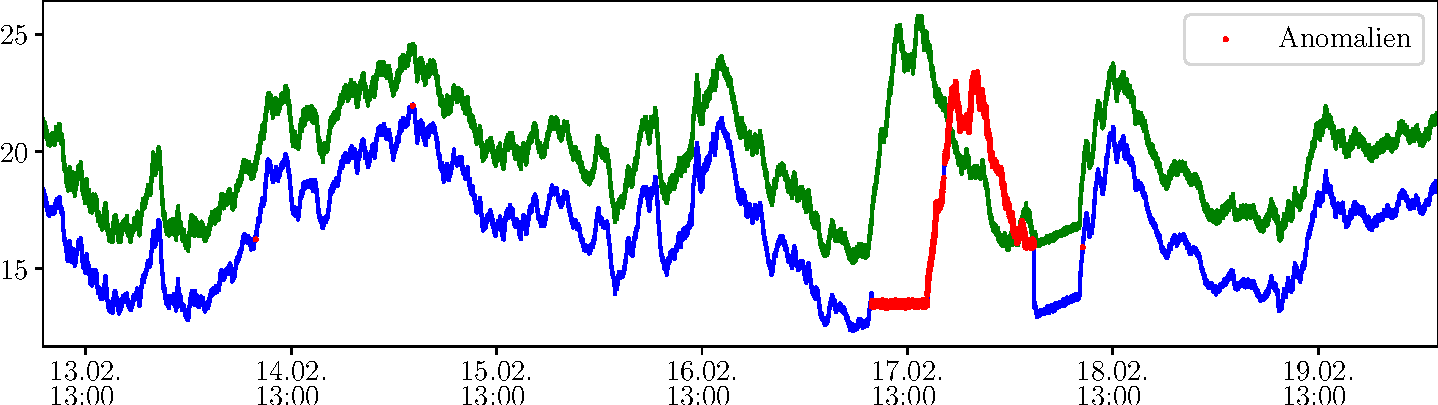
\includegraphics[width=1\linewidth]{ch5_anomalieerkennung/abbildungen/EE_Ergebnis_SOC2.pdf}
    \caption{\centering Visualisierung der Ergebnisse von \acs*{ee} anhand des Testdatensatzes zur \acs{soc} Temperaturanomalie mit zeitlich verzögertem Anstieg im Vergleich mit der \acs{cpu}
    Temperatur. Die rot markierten Punkte stellen die vom Algorithmus detektierten Anomalien dar.}
    \label{fig:EE_bsp_SOC2}
\end{figure}

\section{Kreuzweise Überprüfung der Algorithmen}
In~\hyperref[sec:anomaliearten]{Abs.~\Ref*{sec:anomaliearten}} wurde bereits erwähnt, dass Algorithmen, die für die Detektion bestimmter Anomalien konzipiert
sind, auch in der Detektion eines breiten Spektrums verschiedener Anomalien gut abschneiden. Zur Überprüfung dieser These, die bereits mehrfach dargelegt
werden konnte~\cite[S.~30~-~31]{Wenig2024}~\cite{Schmidl2022}, sollen die selben Algorithmen aus~\hyperref[sec:algorithmen]{Abs.~\Ref*{sec:algorithmen}} deshalb
an allen anderen Datensätzen ebenfalls überprüft werden.

Trotzdem gibt es, bevor die Tests durchgeführt werden, kleine Einschränkungen bzgl.~der Eingangsdaten und damit einhergehenden möglichen Kombinationen. Die
Testdaten, die die Korrelationsanomalien enthalten, können nicht ohne Weiteres an den Algorithmen der Punkt- und Subsequenzanomalien getestet werden, da
diese nur auf univariate Zeitreihen anwendbar sind. Es können zwar multivariate Daten übergeben werden, die dann allerdings univariat verarbeitet werden, also eine
Dimension nach der anderen. Daher scheiden die zur Korrelationsanomaliedetektion generierten Daten aus dem Quervergleich aus. Andersherum sind die Algorithmen
zur Korrelationsanomaliedetektion sehr wohl in der Lage, univariate Daten zu untersuchen und können demnach für alle anderen Testdaten untersucht werden.

Die Detektion von Punkt- und Subsequenzanomalien wurde anhand der drei Algorithmen \ac{swifd}, \ac{md-swifd} und Elliptic Envelope für Punktanomalien und anhand von \ac{hbos}, \ac{swz},
\ac{md-swifd} und Elliptic Envelope für Subsequenzanomalien an den Testdatensätzen aus~\hyperref[fig:punktanomalien_testdata]{Abb.~\Ref*{fig:punktanomalien_testdata}}
durchgeführt und, wie nachfolgend aufgeführt, bewertet. Dabei wurden für alle drei Algorithmen erneut mehrere verschiedene Parameter für die erwartete Kontamination
übergeben. Die \ac{aucpr} Werte aus den jeweiligen Durchläufen werden pro Datensatz gemittelt. Die Ergebnisse der Punktanomaliedetektion liegen
in~\hyperref[tab:punktanomaliedetektion_kreuzweise]{Tab.~\Ref*{tab:punktanomaliedetektion_kreuzweise}} und~\Ref{tab:subsequenzanomaliedetektion_kreuzweise} vor.

\begin{table}[H]
    \centering
    \renewcommand{\arraystretch}{1.5} % Erhöht den Zeilenabstand für bessere Lesbarkeit
    \begin{tabular}{l|lll}
                                & \textbf{\ac{ram} Auslastung}  & \textbf{\ac{cpu} Temperatur}  & \textbf{\ac{cpu} Auslastung} \\
    \hline
    \textbf{\ac{swifd}}         & \cellcolor{red!20}0,07        & \cellcolor{red!35}0,01        & \cellcolor{red!35}0,01 \\
    \textbf{\ac{lstm-ae}}       & \cellcolor{green!7}0,45       & \cellcolor{red!22}0,10        & \cellcolor{green!10}0,50 \\
    \textbf{\ac{md-swifd}}      & \cellcolor{red!20}0,06        & \cellcolor{red!20}0,04        & \cellcolor{red!30}0,02 \\
    \textbf{Elliptic Envelope}  & \cellcolor{green!40}1,0       & \cellcolor{red!5}0,25         & \cellcolor{green!25}0,78 
    \end{tabular}
    \caption{\centering Punktanomaliedetektion durchgeführt mit den Algorithmen zur Detektion der Subsequenz- und Korrelationsanomalien und Bewertung mit \acs*{aucpr}.}
    \label{tab:punktanomaliedetektion_kreuzweise}
\end{table}

\begin{table}[ht]
    \centering
    \renewcommand{\arraystretch}{1.5} % Erhöht den Zeilenabstand für bessere Lesbarkeit
    \begin{tabular}{l|lll}
                                & \textbf{\ac{ram} Auslastung}  & \textbf{\ac{cpu} Temperatur}  & \textbf{Blitzstromaufnahme} \\
    \hline
    \textbf{\ac{swz}}           & \cellcolor{red!17}0,18        & \cellcolor{red!20}0,14        & \cellcolor{red!20}0,14 \\
    \textbf{\ac{hbos}}          & \cellcolor{red!2}0,31         & \cellcolor{red!20}0,15        & \cellcolor{red!20}0,13 \\
    \textbf{\ac{md-swifd}}      & \cellcolor{green!15}0,67      & \cellcolor{green!25}0,75      & \cellcolor{green!30}0,81 \\
    \textbf{Elliptic Envelope}  & \cellcolor{green!30}0,85      & \cellcolor{green!10}0,55      & \cellcolor{red!12}0,2 
    \end{tabular}
    \caption{\centering Subsequenzanomaliedetektion durchgeführt mit den Algorithmen zur Detektion der Punkt- und Korrelationsanomalien und mit \acs*{aucpr} bewertet.}
    \label{tab:subsequenzanomaliedetektion_kreuzweise}
\end{table}

Auffällig ist das gute Abschneiden von \ac{md-swifd} und Elliptic Envelope, die beide zur Detektion von Korrelationensanomalien ausgewählt wurden. Ebenso auffällig
ist das unterschiedlich gute Abschneiden in den Kategorien Punkt- und Subsequenzanomalien. Die Ursache dafür findet sich im grundlegenden Funktionsprinzip der
beiden Algorithmen.

\ac{md-swifd} und Elliptic Envelope detektieren jeweils Anomalien auf Basis der Mahalanobis Distanz, mit dem Unterschied, dass Elliptic Envelope die Mahalanobis Distanz
Punkt für Punkt auf Anomalien untersucht und \ac{md-swifd} den Verlauf der Mahalanobis Distanz in Subsequenzen entspr.~der übergebenen Fenstergröße unterteilt und den
resultierenden Feature Vektor als Basis der Anomaliedetektion verwendet. Aus dem Grund schneidet Elliptic Envelope so gut für Punktanomalien ab, während \ac{md-swifd}
besser für die Detektion von Subsequenzanomalien geeignet ist. Weitere Auffälligkeiten sind auch durch die Natur der Daten zu begründen. Das vergleichbar schlechte
Ergebnis von Elliptic Envelope für den Datensatz der \ac{cpu} Temperatur liegt vor allem am Vorhandensein vieler lokaler Anomalien, während die anderen beiden
Datensätze zur \ac{ram} und \ac{cpu} Auslastung rein globale Anomalien aufweisen.

Die Mahalanobis Distanz einer Zeitreihe basiert allgemein gem.~\hyperref[eq:mahalanobis_dist]{Gl.~\Ref*{eq:mahalanobis_dist}} auf der inversen Kovarianzmatrix der
Zeitreihe. Liegt die Zeitreihe in nur einer Dimension vor, ist die Kovarianzmatrix nur noch eine Matrix der Form $1\times 1$ und somit ein Skalar, wonach sich die
Mahalanobis Distanz einer univariaten Zeitreihe vereinfachen lässt und dem Z-Score entspricht, was das Finden lokaler Anomalien als besonders schwierig gestaltet,
da sie nur im unmittelbaren Kontext anomal sind (vgl.~\hyperref[sec:punktanomalien]{Abs.~\Ref*{sec:punktanomalien}}).

Im Gegensatz dazu ermöglicht die Subsequenzanalyse der Mahalanobis Distanz in \ac{md-swifd} das Finden ungewöhnlicher Muster, da auch die Feature Vektoren ungewöhnlicher
Subsequenzen im Vergleich zu allen anderen, normalen Subsequenzen vom Isolation Forest Algorithmus detektiert werden können.

Die Ergebnisse für \ac{lstm-ae} lassen vermuten, dass der Algorithmus nur begrenzt dafür geeignet ist, Punktanomalien zu entdecken. Dieser Eindruck ist bedingt
durch die Art, wie Precision, Recall und folglich \ac{aucpr} zustande kommen. Es wird Punkt für Punkt verglichen, ob ein Punkt entweder in die Kategorie True Positive,
False Positive, True Negative oder False Negative gehört. Damit der \ac{lstm-ae} in der Lage ist, sowohl globale als auch lokale Anomalien zu detektieren,
wird über mehrere Sequenzlängen iteriert und die Anomaliebewertungen gemittelt. Kurze Sequenzen der Länge 1 detektieren globale Anomalien zuverlässig, während für
lokale Anomalien Sequenzen mit ca. 5 oder mehr Datenpunkten benötigt werden, um diese zu detektieren. Die Folge ist, dass auch direkt angrenzende Indizes aufgrund der
Länge der Sequenz mit einem Rekonstruktionsfehler belastet werden, und entsprechend der Schwelle auch als Anomalie eingestuft werden. Diese Unsicherheit spiegelt sich
im \ac{aucpr} Wert wider und ist auch in~\hyperref[fig:lstmae_points_mse]{Abb.~\Ref*{fig:lstmae_points_mse}} an zwei einzelnen Punktanomalien aus dem Testdatensatz zur
CPU Auslastung aus~\hyperref[fig:punktanomalien_testdata]{Abb.~\Ref*{fig:punktanomalien_testdata}} dargestellt.

\begin{figure}[H]
    \centering
        \includegraphics[width=1\linewidth]{ch5_anomalieerkennung/abbildungen/LSTMAE_POINTS_erklärung.pdf}
    \caption{\centering Ausschnitt aus der Ausgabesequenz des \acs*{lstm-ae} nach Analyse des Datensatzes der \acs*{cpu} Auslastung
    aus~\hyperref[fig:punktanomalien_testdata]{Abb.~\Ref*{fig:punktanomalien_testdata}} mit rot markiertem Index der tatsächlichen Punktanomalie. Zu sehen ist der
    Grund für den suboptimalen \acs*{aucpr} Wert, obwohl die Anomalie grundätzlich gefunden werden kann. Aufgrund der Iteration über mehrere Sequenzlängen sind Punkte
    um die gefundene Anomalie herum ebenfalls mit einem Score $>$ 0 versehen.}
    \label{fig:lstmae_points_mse}
\end{figure}

Das Beispiel zeigt, dass sich~\ac{lstm-ae} trotz der nicht optimalen \ac{aucpr} Bewertung gut zur Punktanomaliedetektion
eignet.~\hyperref[fig:lstmae_points_CPU]{Abb.~\Ref*{fig:lstmae_points_CPU}} macht dies anhand der rot markierten Bereiche deutlich. Die Detektion ist also nicht
perfekt, aber es wird deutlich, dass der Algorithmus den unmittelbaren Bereich einer Punktanomalie genau detektieren kann. Für weitere Betrachtungen soll diese
Feststellung völlig ausreichen, denn vor einem tatsächlichen Wartungseinsatz wird eine gefundene Anomalie nochmal überprüft und kann dementsprechend eingeordnet
werden.

\begin{figure}[htbp]
    \centering
        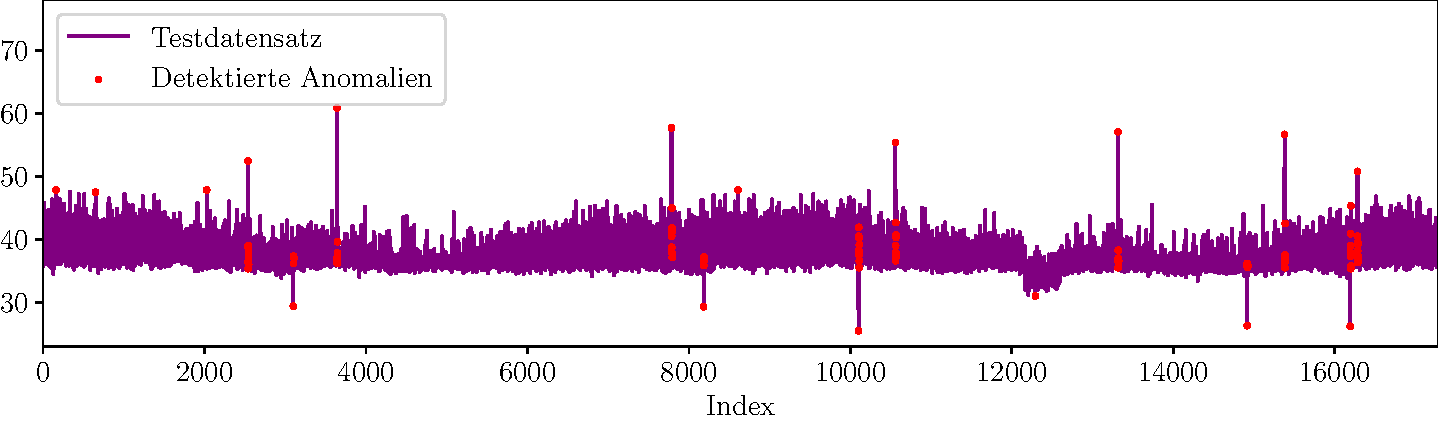
\includegraphics[width=1\linewidth]{ch5_anomalieerkennung/abbildungen/LSTMAE_POINTS_CPU_beispiel.pdf}
    \caption{\centering Gesamter Datensatz zur CPU Auslastung mit markierten Punktanomalien, die von \acs*{lstm-ae} gefunden wurden.}
    \label{fig:lstmae_points_CPU}
\end{figure}

\section{Diskussion der Ergebnisse}
Im Laufe des Kapitels hat sich die Unsicherheit der Testergebnisse aufgrund der Imperfektionen der Testdatensätze sowie der Evaluationsmetriken aufgetan. Diese
lassen zwar keine absolute und zweifelsfreie Beurteilungen der getesteten Algorithmen zu, aber sie sollen trotzdem nicht verhindern, dass die Performance mit Stärken
und Schwächen der einzelnen Algorithmen offen gelegt werden konnten. Der Punkt-für-Punkt-Ansatz der gewählten Metriken Precision, Recall und \ac{aucpr} sorgen dafür,
dass Algorithmen auf den ersten Blick ein schlechteres Ergebnis erzielen als es ein zweiter, genauerer Blick zeigt.

Eine absolute Beurteilung sollte auch nicht das Ziel der Evaluation sein, sondern lediglich ein Hilfsmittel zur besseren Vergleichbarkeit auch im Hinblick auf
mögliche Abhängigkeiten bezüglich der Parameter.